%%
%% This is file `sample-sigconf.tex',
%% generated with the docstrip utility.
%%
%% The original source files were:
%%
%% samples.dtx  (with options: `sigconf')
%% 
%% IMPORTANT NOTICE:
%% 
%% For the copyright see the source file.
%% 
%% Any modified versions of this file must be renamed
%% with new filenames distinct from sample-sigconf.tex.
%% 
%% For distribution of the original source see the terms
%% for copying and modification in the file samples.dtx.
%% 
%% This generated file may be distributed as long as the
%% original source files, as listed above, are part of the
%% same distribution. (The sources need not necessarily be
%% in the same archive or directory.)
%%
%% The first command in your LaTeX source must be the \documentclass command.
\documentclass[sigconf,nonacm]{acmart}


%%
%% \BibTeX command to typeset BibTeX logo in the docs
\AtBeginDocument{%
  \providecommand\BibTeX{{%
    \normalfont B\kern-0.5em{\scshape i\kern-0.25em b}\kern-0.8em\TeX}}}

%% Rights management information.  This information is sent to you
%% when you complete the rights form.  These commands have SAMPLE
%% values in them; it is your responsibility as an author to replace
%% the commands and values with those provided to you when you
%% complete the rights form.
\setcopyright{acmcopyright}
\copyrightyear{2020}
\acmYear{2020}
\acmDOI{}
\makeatletter
\renewcommand\@formatdoi[1]{\ignorespaces}
\makeatother

%% These commands are for a PROCEEDINGS abstract or paper.
\acmConference{}
\acmBooktitle{Determination of Alcohol Consumption Level Using Smartphone Data,
  July 22, 2020, Bremen, Germany}
\acmPrice{}
\acmISBN{}
\usepackage{todonotes}

\usepackage{graphicx}
\graphicspath{ {./figures/} }

\usepackage{subcaption}
% for figures: caption label is italic, the caption text is bold / italic
%\captionsetup[figure]{labelfont=it,textfont={bf,it}}
\captionsetup[figure]{justification=raggedright,singlelinecheck=false}

% for subfigures: caption label is bold, the caption text normal.
% justification is raggedright (i.e. left aligned)
% singlelinecheck=off means that the justification setting is used even when the caption is only a single line long. 
% if singlelinecheck=on, then caption is always centered when the caption is only one line.
\captionsetup[subfigure]{labelfont=bf,textfont=normalfont,singlelinecheck=off,justification=raggedright}


\usepackage{siunitx}


\usepackage{hyperref}

\usepackage{stfloats}

%%
%% Submission ID.
%% Use this when submitting an article to a sponsored event. You'll
%% receive a unique submission ID from the organizers
%% of the event, and this ID should be used as the parameter to this command.
%%\acmSubmissionID{123-A56-BU3}

%%
%% The majority of ACM publications use numbered citations and
%% references.  The command \citestyle{authoryear} switches to the
%% "author year" style.
%%
%% If you are preparing content for an event
%% sponsored by ACM SIGGRAPH, you must use the "author year" style of
%% citations and references.
%% Uncommenting
%% the next command will enable that style.
%%\citestyle{acmauthoryear}

%%
%% end of the preamble, start of the body of the document source.
\begin{document}

%%
%% The "title" command has an optional parameter,
%% allowing the author to define a "short title" to be used in page headers.
\title{Determination of Alcohol Consumption Level Using Smartphone Data}

%%
%% The "author" command and its associated commands are used to define
%% the authors and their affiliations.
%% Of note is the shared affiliation of the first two authors, and the
%% "authornote" and "authornotemark" commands
%% used to denote shared contribution to the research.
\author{twsl}
\email{45483159+twsl@users.noreply.github.com}
\affiliation{%
	\institution{University of Bremen}
	\city{Bremen}
	\state{Germany}
}

\author{holysh1t}
\email{30555166+holysh1t@users.noreply.github.com}
\affiliation{%
	\institution{University of Bremen}
	\city{Bremen}
	\state{Germany}
}

\author{hiraad}
\email{35299559+hiraad@users.noreply.github.com}
\affiliation{%
	\institution{University of Bremen}
	\city{Bremen}
	\state{Germany}
}

\author{dast96}
\email{66383908+dast96@users.noreply.github.com}
\affiliation{%
	\institution{University of Bremen}
	\city{Bremen}
	\state{Germany}
}

%%
%% By default, the full list of authors will be used in the page
%% headers. Often, this list is too long, and will overlap
%% other information printed in the page headers. This command allows
%% the author to define a more concise list
%% of authors' names for this purpose.
\renewcommand{\shortauthors}{twsl, holysh1t, hiraad and dast96}

%%
%% The abstract is a short summary of the work to be presented in the
%% article.
\begin{abstract}
	It's the unfortunate reality that people drive under the influence of alcohol, leading to accidents, which may result in injuries and even fatalities.
	With modern technology such as smartphones becoming a norm in the current day and age, it is a responsible decision to exploit the power of technology to avoid human disasters and prevent fatalities.
	In our paper, we aim to do just that by following an approach that seeks to determine the alcohol consumption level using smartphone data and identify how our ensemble methods compare to the performance of the methods discussed in \textit{Learning to Detect Heavy Drinking Episodes Using Smartphone Accelerometer Data} \cite{DBLP:conf/ijcai/KillianPNMC19}.
	To achieve this, we used the available accelerometer data from the smartphone to create a regression model that predicts the transdermal alcohol concentration.
	For the preparation of the data set, we used various methods such as interpolation, and splitting the data into sets containing only valid data.
	To optimize our machine learning model, we extracted features with sliding windows. Our best regression model presented a result with 0.0058061 mean squared error but it did not match our expectations.
\end{abstract}

%%
%% Keywords. The author(s) should pick words that accurately describe
%% the work being presented. Separate the keywords with commas.
\keywords{drinking, accelerometer data, smartphone, alcohol detection, smartphone data, sliding windows, regressor, machine learning, optuna optimize}

%% A "teaser" image appears between the author and affiliation
%% information and the body of the document, and typically spans the
%% page.

%%
%% This command processes the author and affiliation and title
%% information and builds the first part of the formatted document.
\maketitle


\section{Introduction}

It's the unfortunate reality that people drive under the influence of alcohol, which leads to accidents that cause injuries and even fatalities. In the age of digitalization, smartphones are becoming more and more the norm. 
Therefore, it is a responsible decision to take advantage of this technology to prevent people from driving under the influence of alcohol.
In 85\% of car accidents in Germany causing personal injury, at least one person was under the influence of alcohol \cite{destatis}.
In addition, 4.5\% of all car accidents in Germany are accidents due to alcohol \cite{statista}.
To reduce the amount of accidents with alcohol involved, we propose the usage of accelerometer data as an additional indicator  of alcohol consumption level.

We used a prerecorded dataset, which consists of smartphone accelerometer and transdermal alcohol concentration (TAC) data.
In order to decrease the amount of drunk driving accidents, we aim to train a regressor model that predicts when someone is about to exceed the legally allowed alcohol level.
On the other hand, such a solution comes with a great responsibility of protecting people's personal information, as some companies may target vulnerable users with more specific ads, insurance companies may raise the monthly bill for reckless drinking and driving under the influence.
Drunk shopping is an enormous industry and further highlights the significance of responsible acting regarding our topic at hand.
\begin{quote}
	``Retailers go to great lengths to capitalize on your drunken stupor and capture a chunk of this ~\$45B market'' \cite{hustle}
\end{quote}

Even tho \citeauthor{DBLP:conf/ijcai/KillianPNMC19} in \cite{DBLP:conf/ijcai/KillianPNMC19} decided to use a binary prediction formulation rather than a regression formulation, because of the high variance of the accuracy of the \texttt{SCRAM} sensors, we wanted a solution that is not trained on a specific legal limit, and therefore can easily be adopted all over the world regardless of local the laws concerning the legal limit of alcohol consumption. Nonetheless, using the same dataset as \citeauthor{DBLP:conf/ijcai/KillianPNMC19}, we expect to achieve better performance by using a regression formulation for the problem at hand.

\section{Background}
The dataset used was downloaded from the UCI Machine Learning Repository \cite{Dua:2019} and is owned by \citeauthor{DBLP:conf/ijcai/KillianPNMC19} \cite{DBLP:conf/ijcai/KillianPNMC19}.
It contains three-axis time series accelerometer data from mobile phones and time series TAC data, which is a real-time measure of intoxication collected through the skin and was collected by a \texttt{SCRAM} ankle bracelet.
All data is fully anonymized.
A total of 20 undergrad students, 10 men and 10 women, each in their senior year, were recruited. The recordings were taking during a bar crawl.
One participant couldn't install the application, such that no accelerometer data was recorded and the TAC readings for an additional six participants were deemed unusable by \texttt{SCRAM}.
The accelerometer readings were collected at $40 \si{\hertz}$ by a self made application and periodically send to an InfluxDB server.
The data was collected from a mix of $11$ iOS and $2$ Android phones.
Meanwhile, the TAC readings were collected at $30\si{\minute}$ intervals.

Using the IR Voltage and the temperature, cleaned time-series TAC data was calculated from these raw readings.
The cleaned TAC readings were processed with a zero-phase low-pass filter to smooth noise without shifting phase, then were shifted backwards by 45 minutes such that the labels more closely match the true intoxication of the participant, since alcohol takes about 45 minutes to exit through the skin.
Cleaned TAC readings which are more readily usable for processing have two columns: a timestamp and TAC reading. 
This results in $14 057 567$ accelerometer readings and $715$ TAC readings for a total of 13 participants.
The TAC is measured in grams per deci liter where $0.08 \frac{\si{\gram}}{\si{\deci\litre}}$ is the legal limit for intoxication while driving in California and $0.05 \frac{\si{\gram}}{\si{\deci\litre}}$ in Germany.

In the end there are three sets of data: three-axis time-series accelerometer, the cleaned time-series TAC and the uncleaned time-series TAC data.
For further details on how the data was processed see the original paper \cite{DBLP:conf/ijcai/KillianPNMC19}.

For this particular use-case the usage of \texttt{SCRAM} ankle bracelets was unproblematic, but generally speaking, especially with regards to law enforcement and the current Covid pandemic, the evaluation is prone to faults by disinfectants containing alcohol like hand sanitizers and even tiny alcohol splashes. These events can falsify the readings of the aforementioned ankle bracelet. 

The National Highway Traffic Safety Administration deemed the technology of transdermal alcohol measuring valid, but ``the actual equipment with false-negatives rates [...] are too high'' \cite{nhtsa_scram}. 




\section{Exploratory Data Analysis}
The three sets of data explained in the last section were composed of one large, accelerometer dataset that contained data points for all the participants.
And the remaining two were a raw and clean version of the TAC data per participant.
In order to extract more features we had to merge the three sets into one complete dataset.
The data needed some preprocessing, before feature extraction, which is the purpose of this section.
The accelerometer sets (Figure \ref{fig:acc-comp}) for one, sampled at $40 \si{\hertz}$ contained many more points as opposed to the data from the bracelets (Figure \ref{fig:tac-comp}), captured once every $30$ minutes.
Another problem was that the accelerometer data often contained gaps for various reasons including phone power outages.
\begin{figure}[h]
	\begin{subfigure}[c]{0.49\columnwidth}
		\centering
		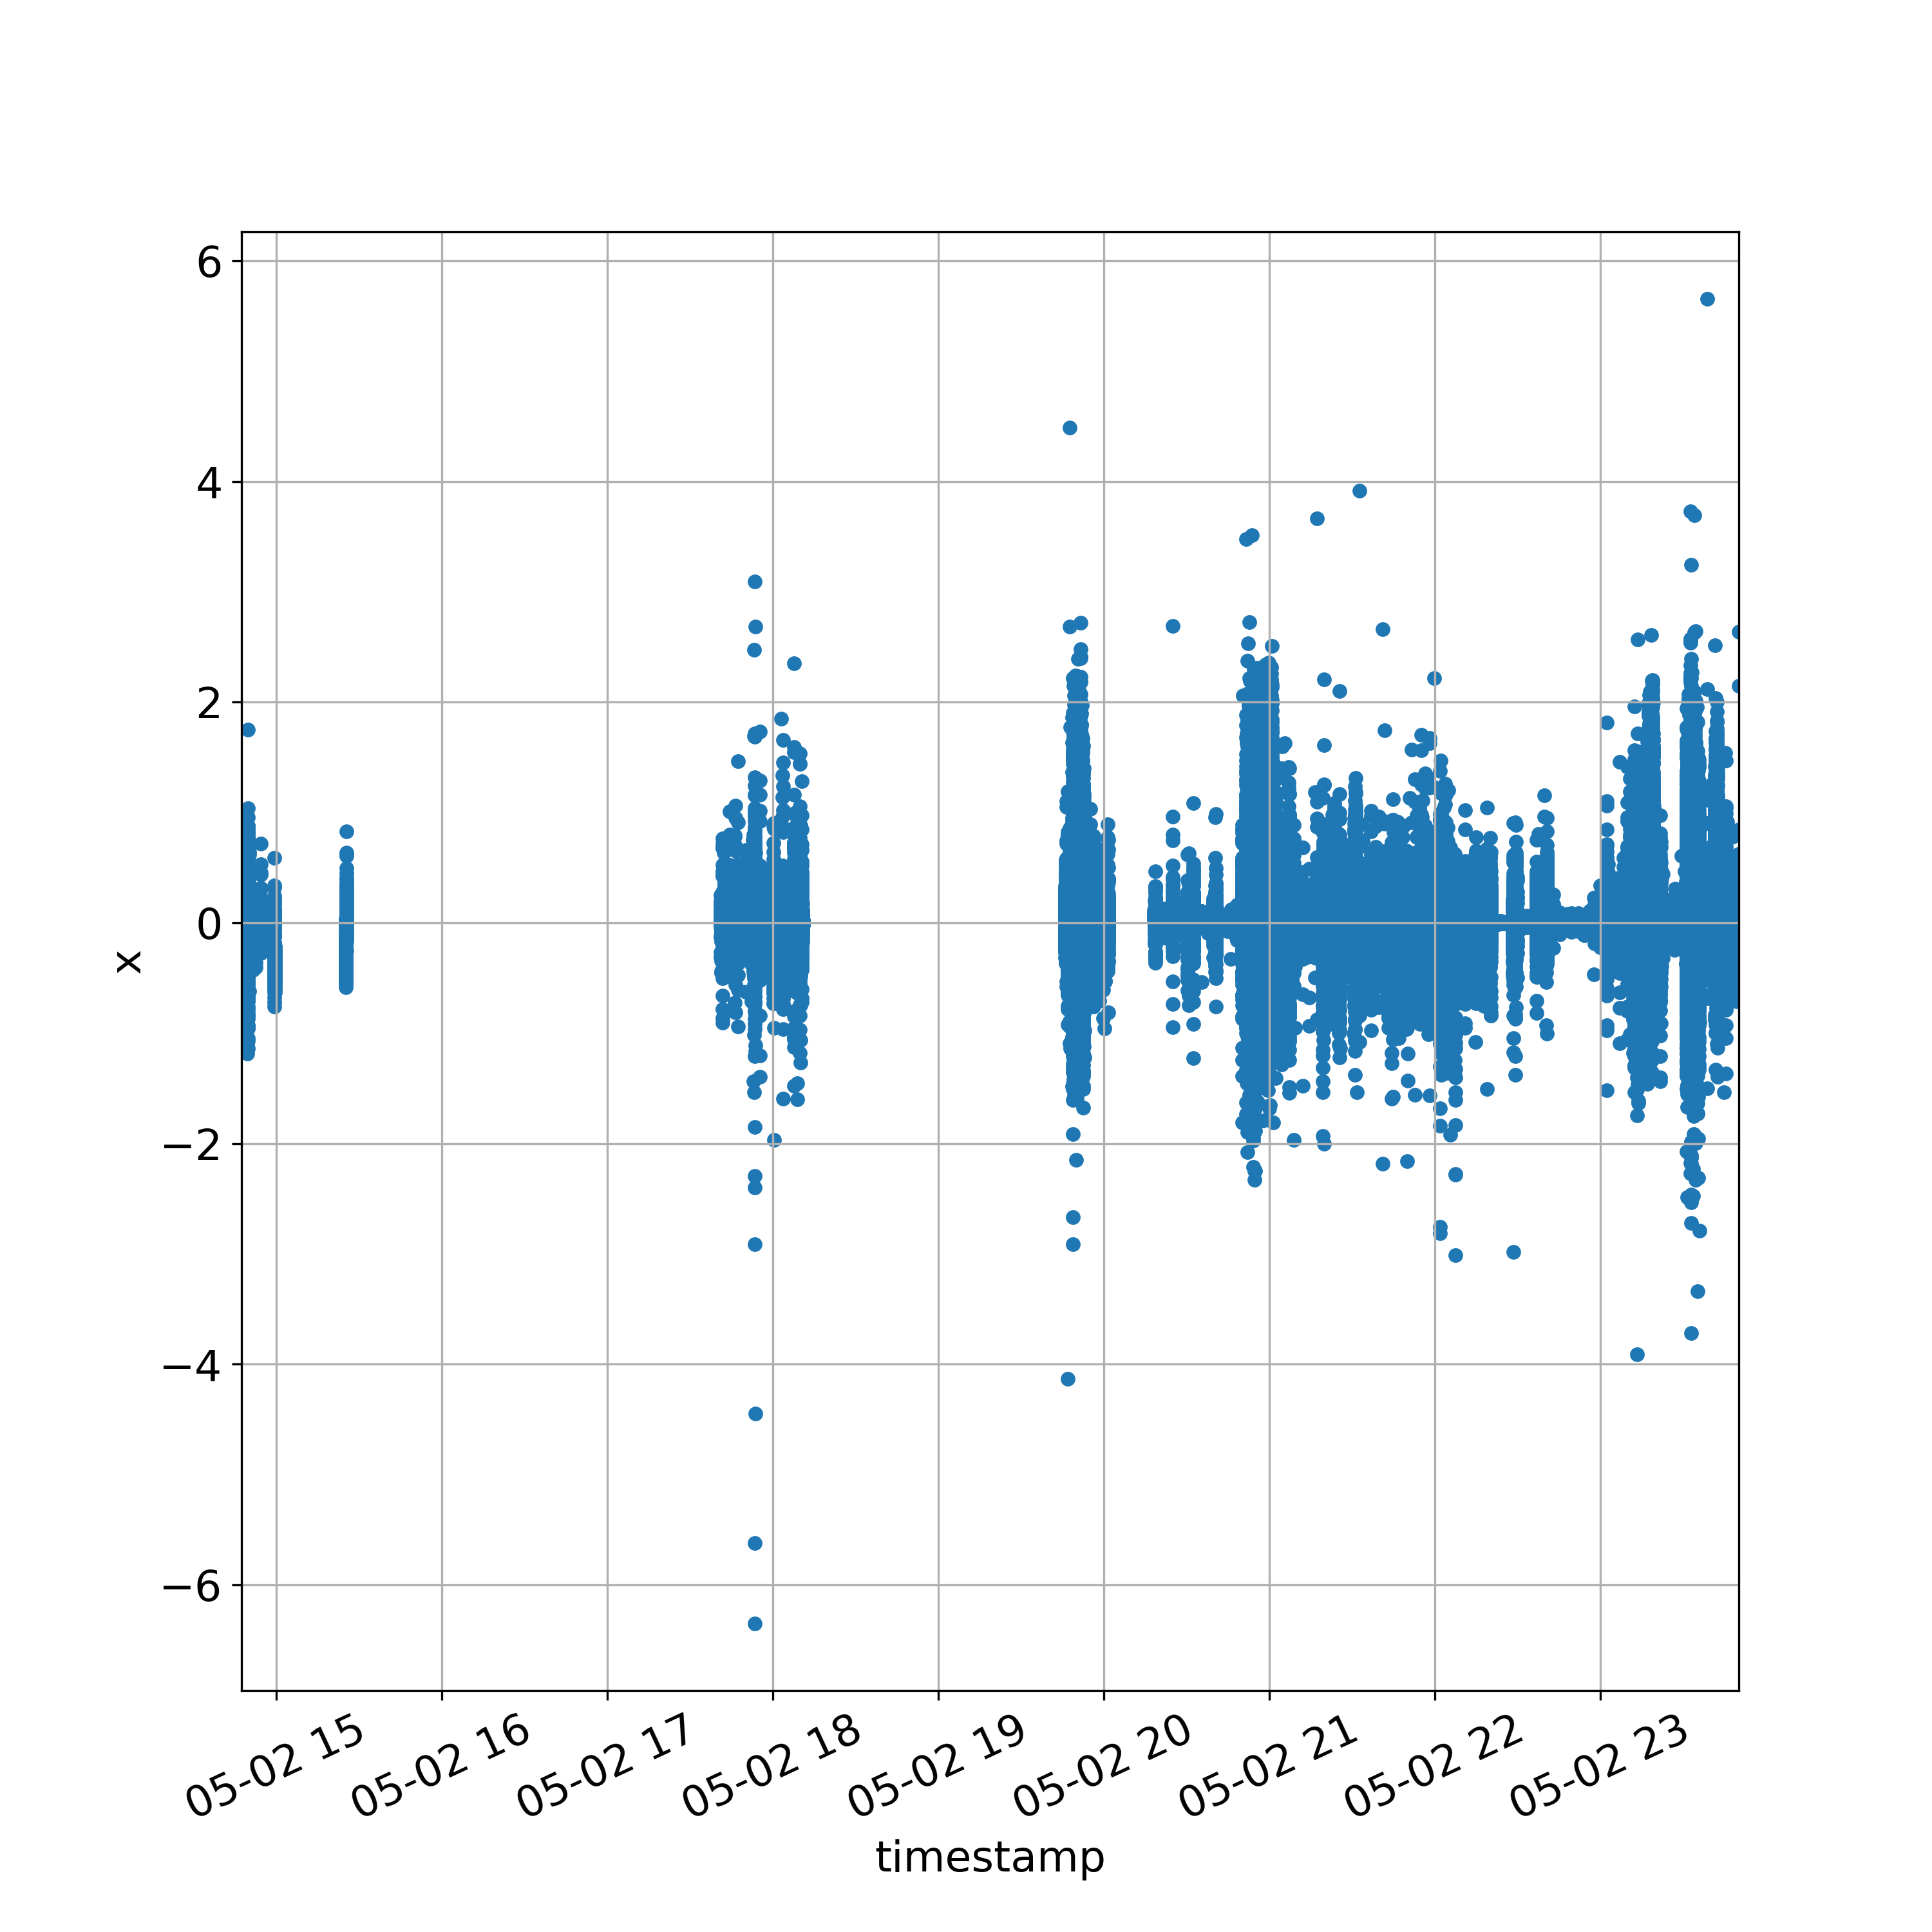
\includegraphics[width=\textwidth]{DC6359_acc_x}
		\caption{Original}
		\label{fig:acc-orig}		
	\end{subfigure}\hfill%
	\begin{subfigure}[c]{0.49\columnwidth}
		\centering
		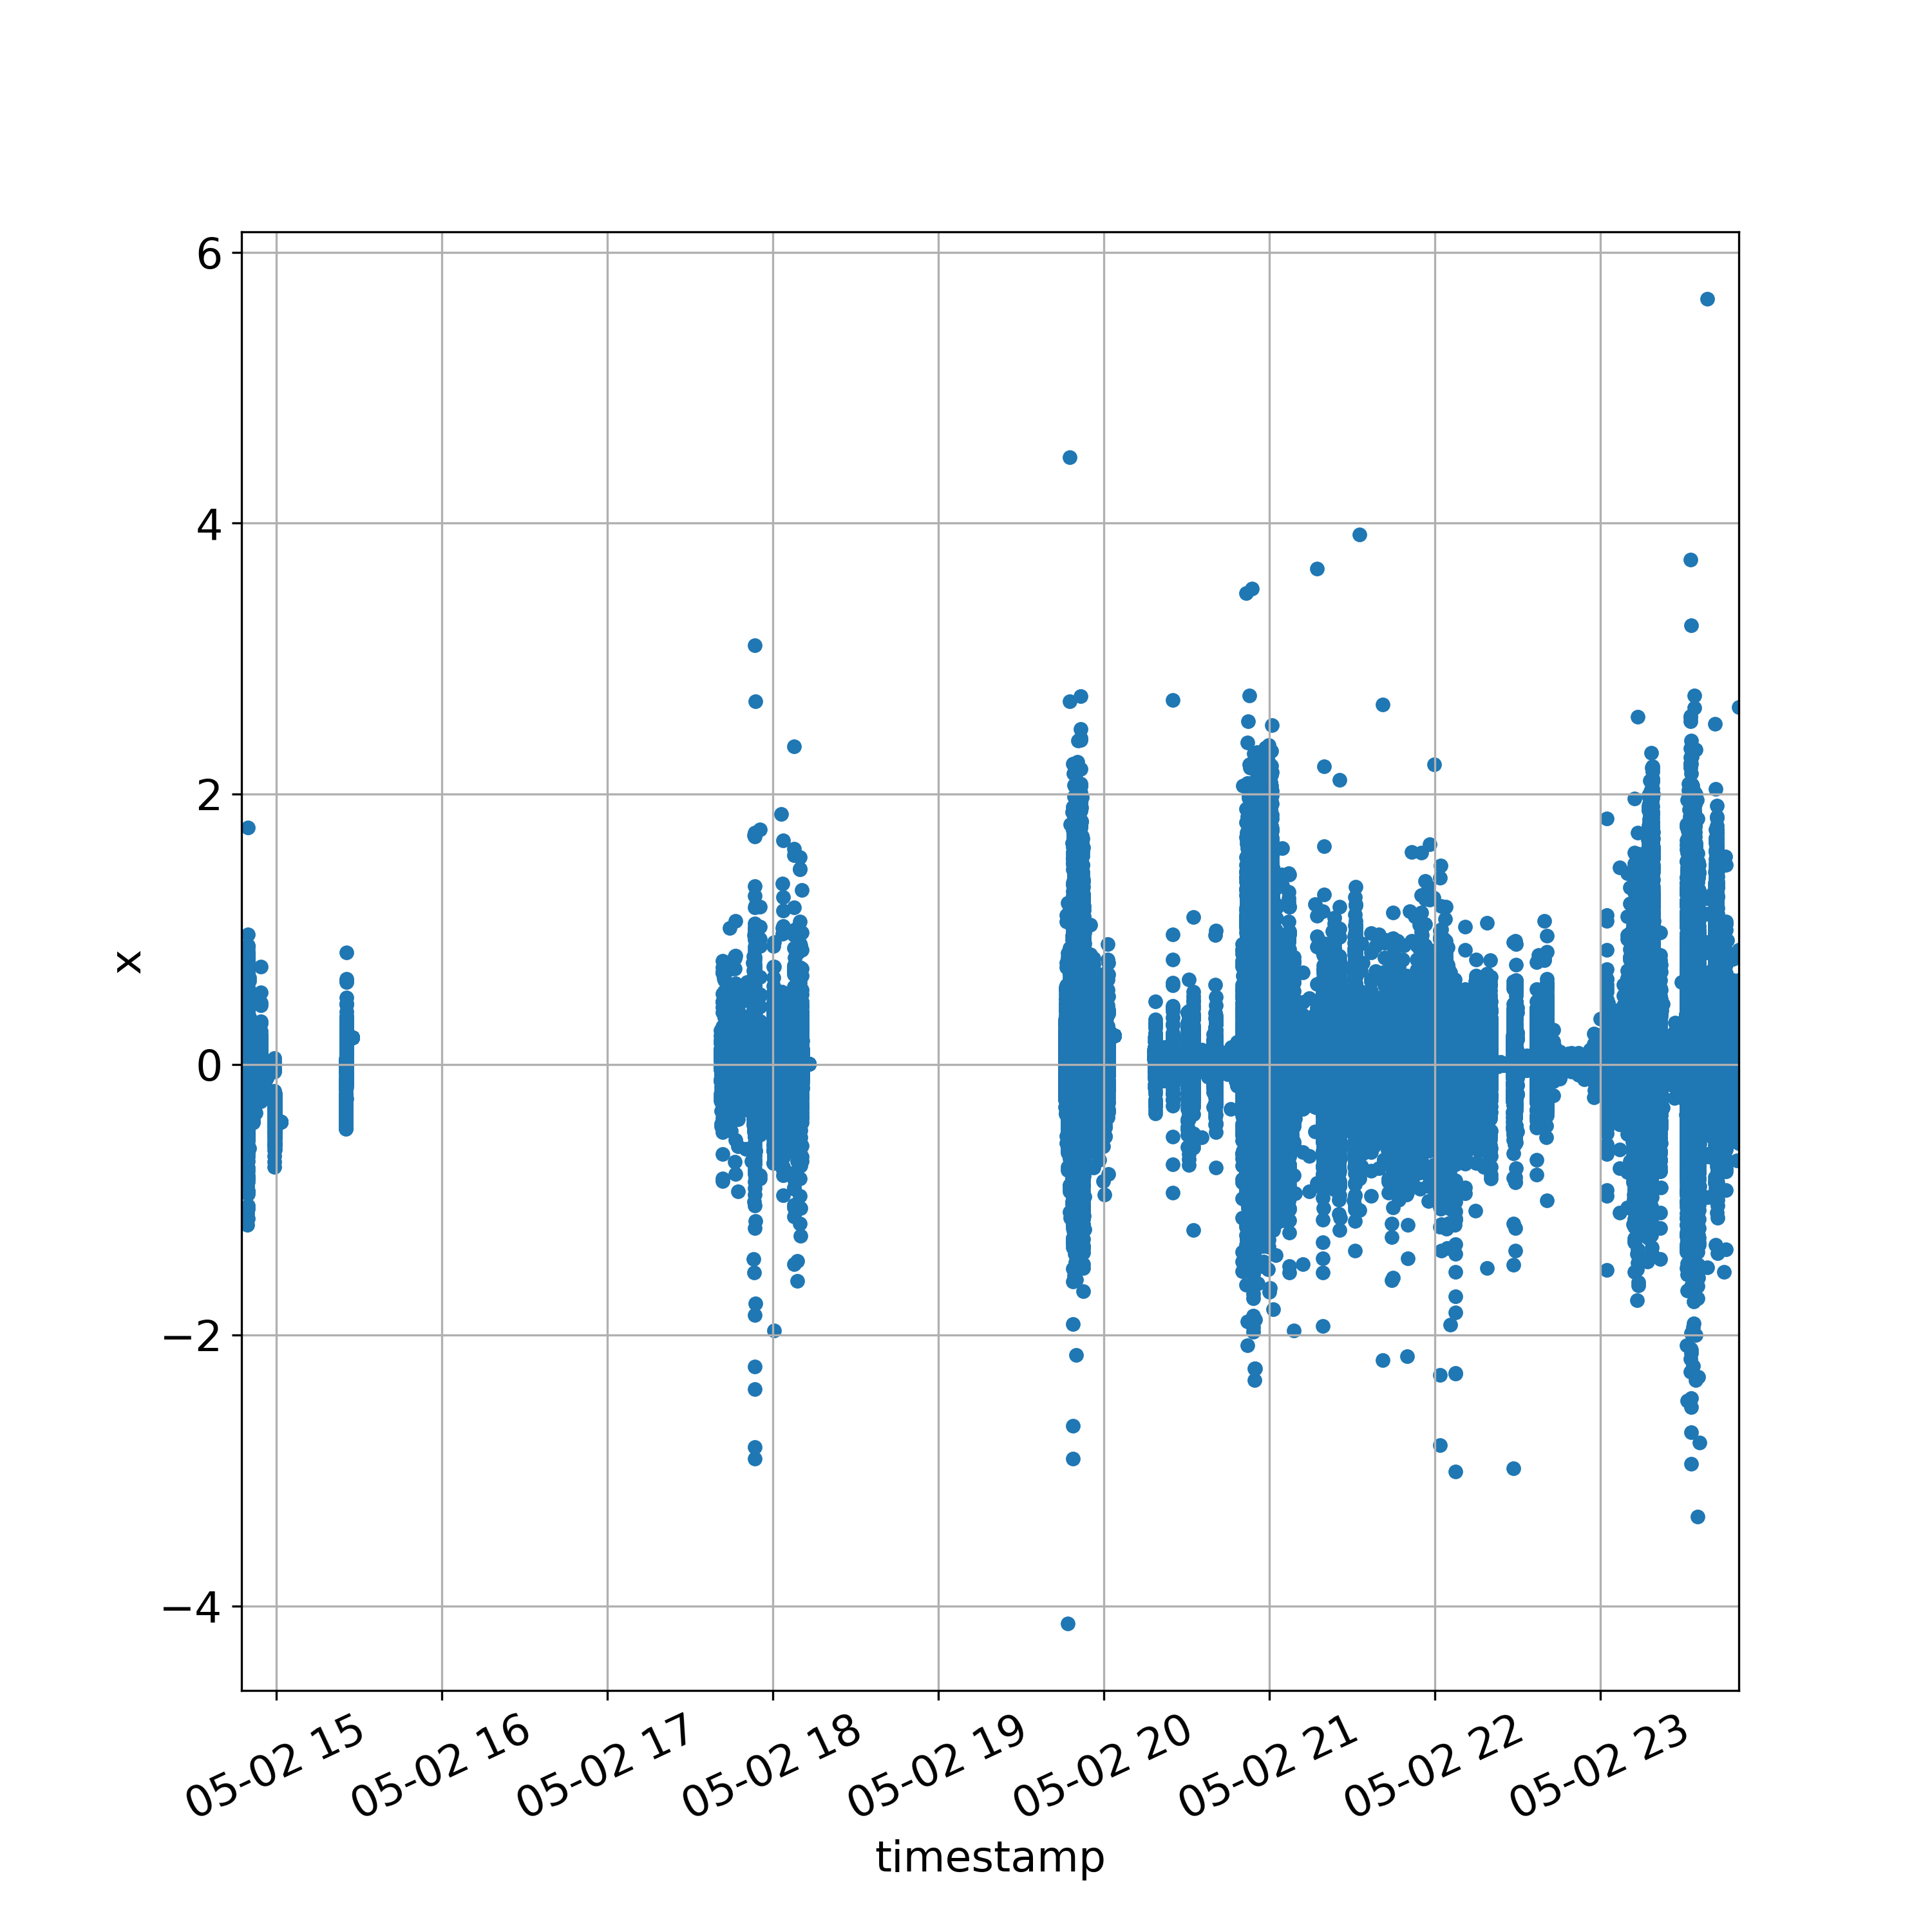
\includegraphics[width=\textwidth]{DC6359_merged_x}
		\caption{Resampled and interpolated}
		\label{fig:acc-intpl}
	\end{subfigure}
	\caption{Comparison of accelerometer data for sample \texttt{DC6359}}
	\label{fig:acc-comp}
\end{figure}
\begin{figure}[h]
	\begin{subfigure}[c]{0.49\columnwidth}
		\centering
		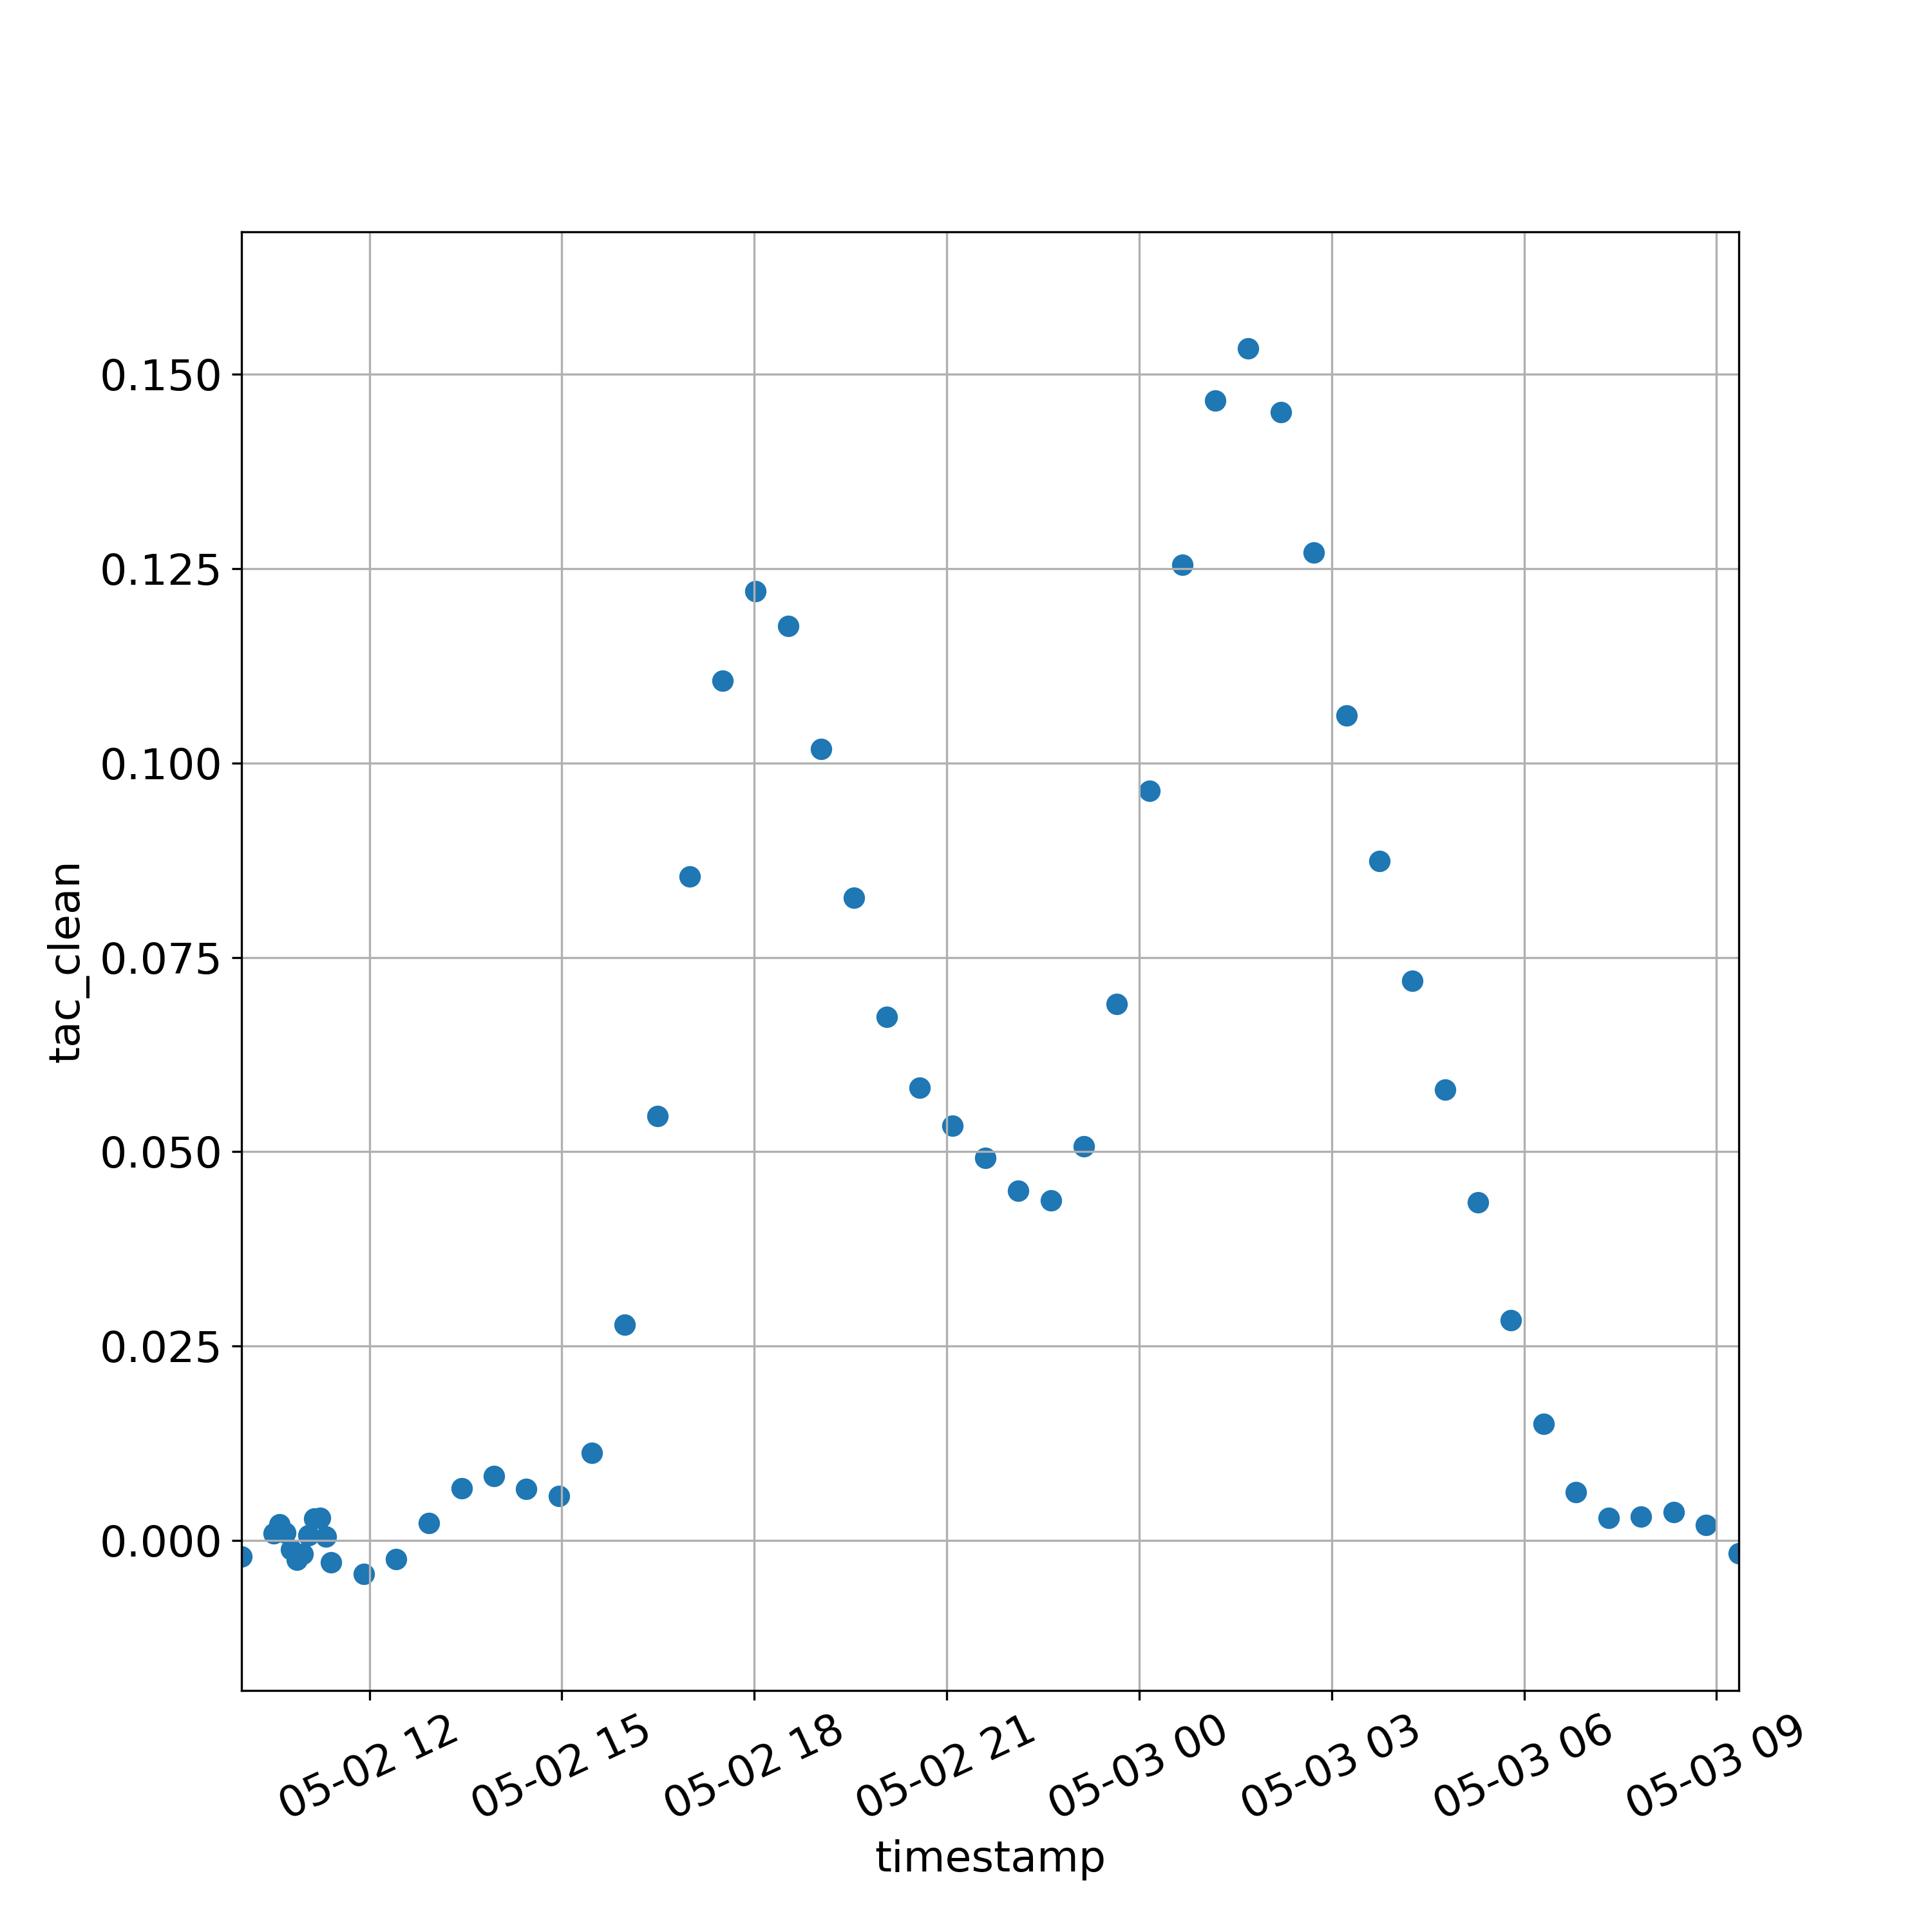
\includegraphics[width=\textwidth]{DC6359_tac_clean}
		\caption{Original}
		\label{fig:tac-orig}		
	\end{subfigure}\hfill%
	\begin{subfigure}[c]{0.49\columnwidth}
		\centering
		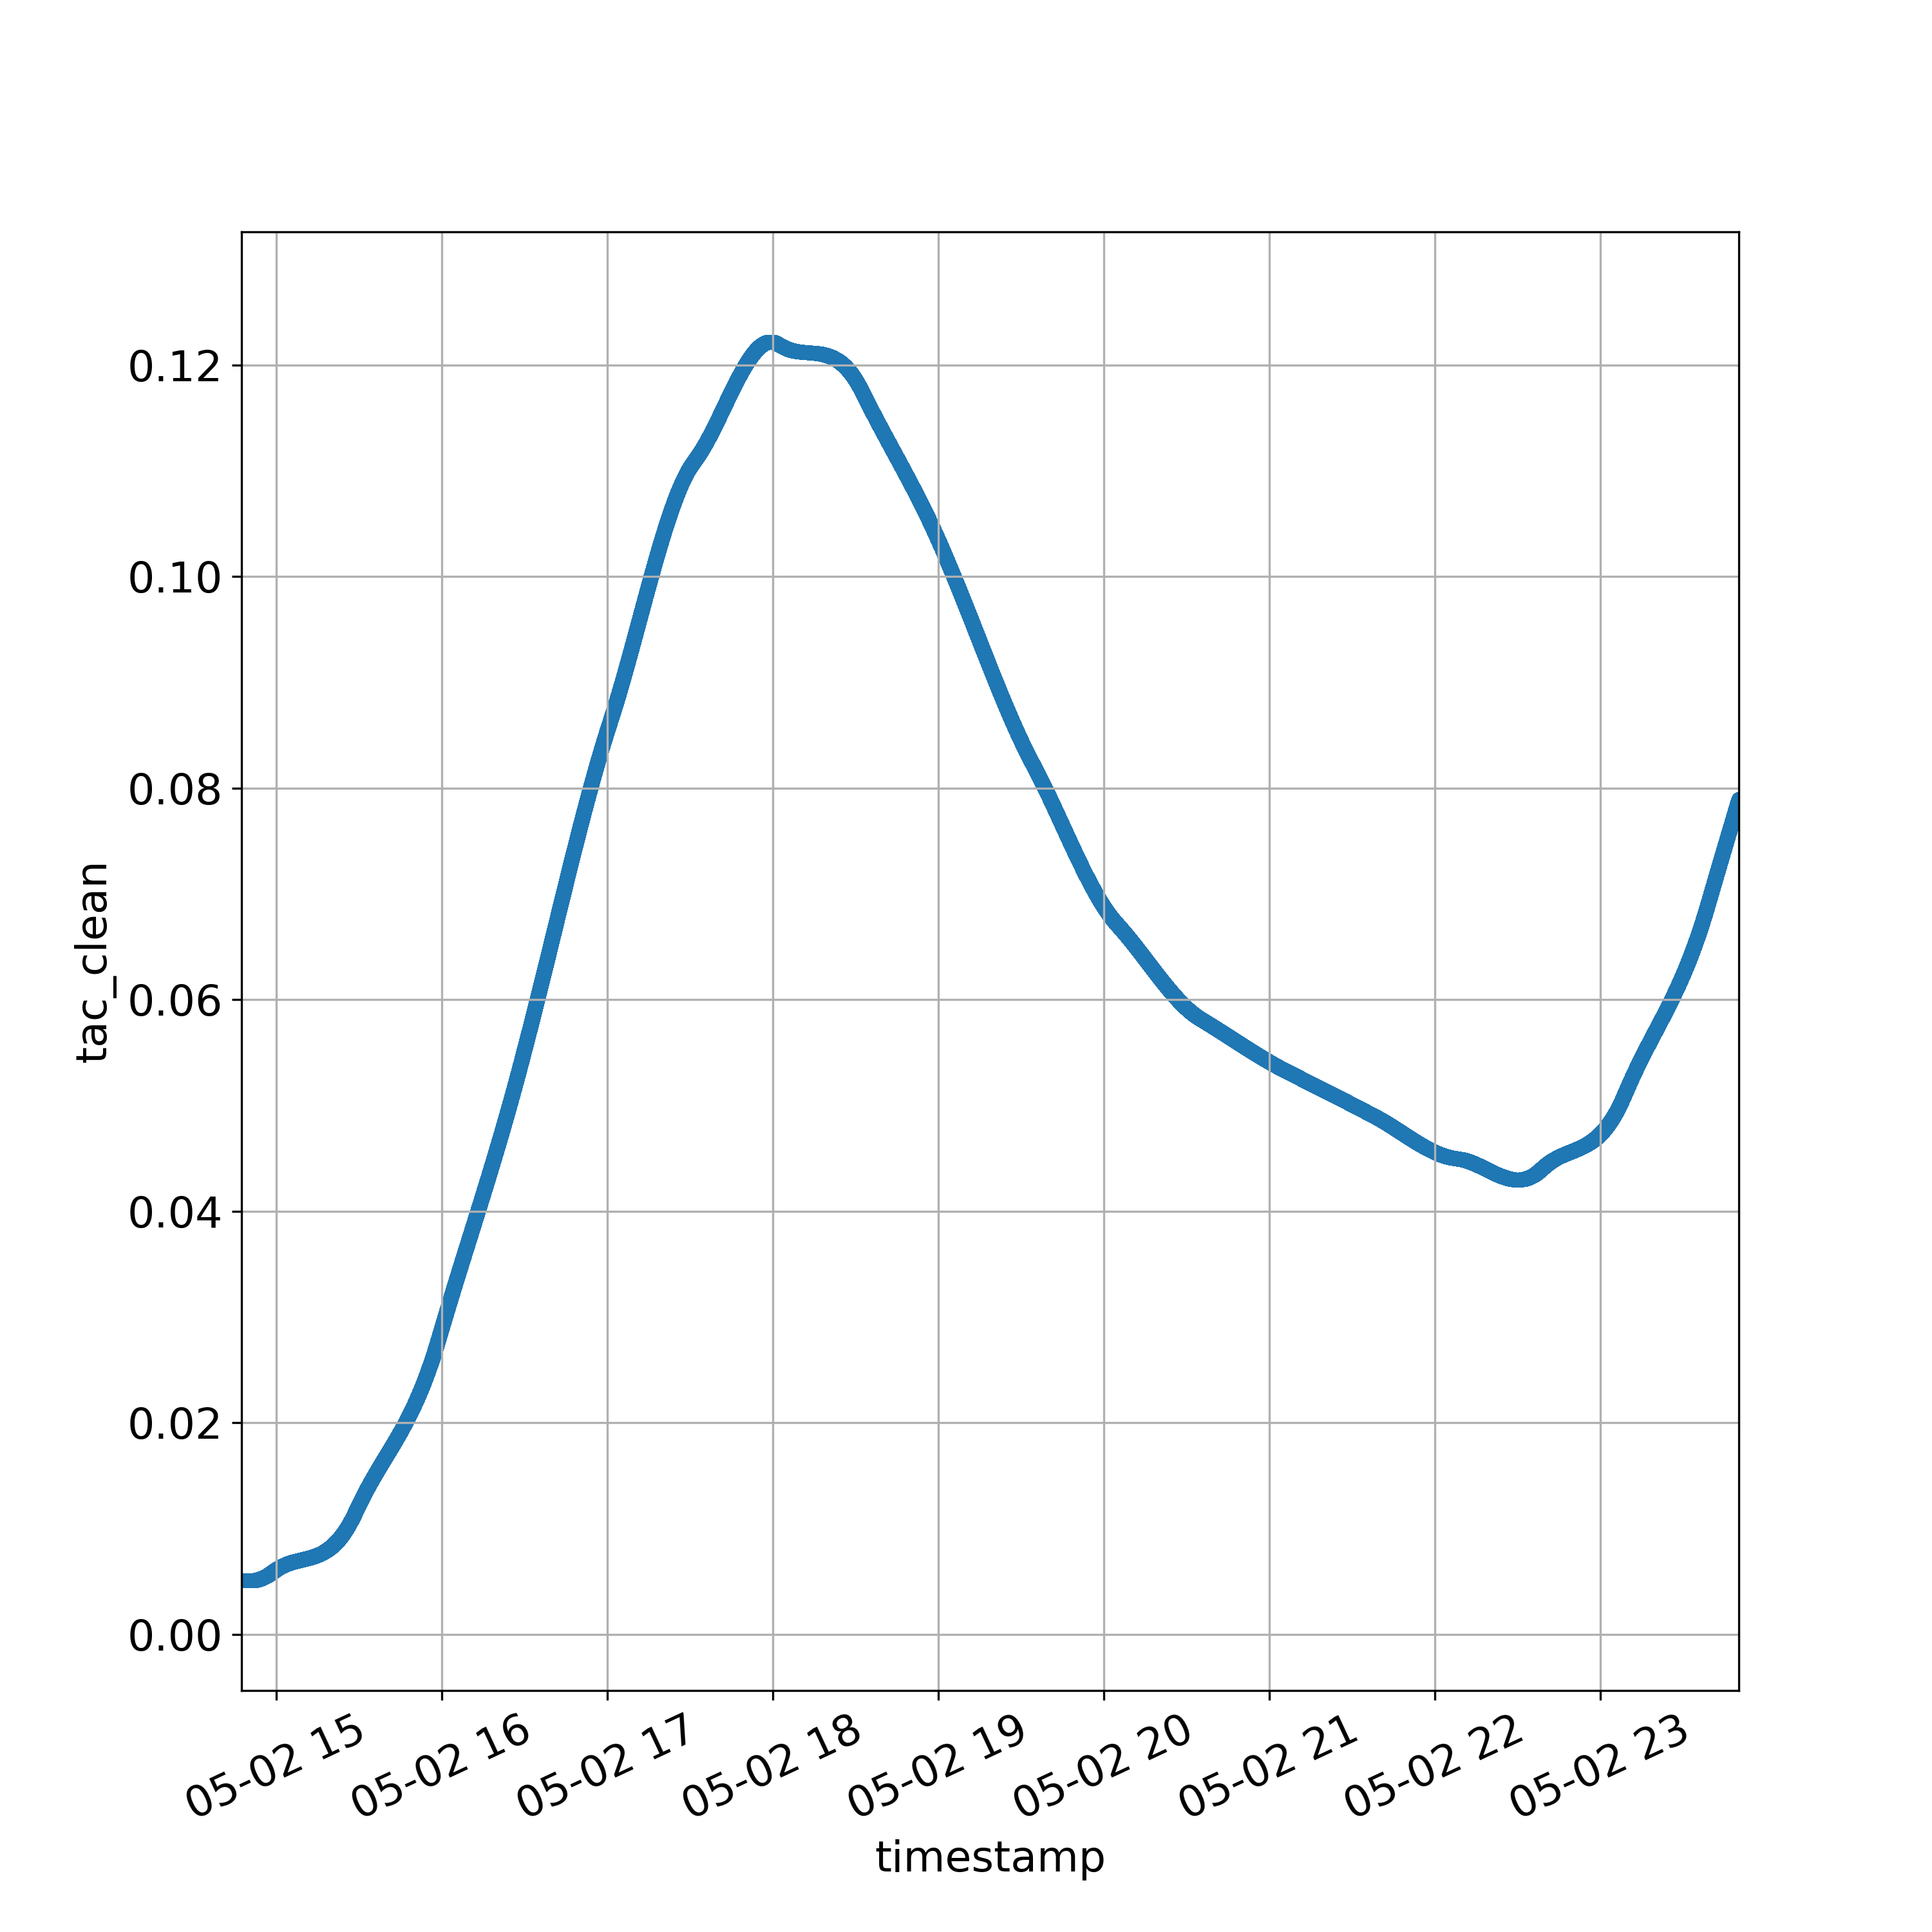
\includegraphics[width=\textwidth]{DC6359_merged_clean}
		\caption{Cropped, resampled and interpolated}
		\label{fig:tac-intpl}
	\end{subfigure}
	\caption{Comparison of TAC data for sample \texttt{DC6359}}
	\label{fig:tac-comp}
\end{figure}
We splitted accelerometer data to contain points for each user independently and then merged raw and clean TAC datasets together to have both attributes into one set before a final combination of all three.
In order to prevent target leakage and the raw readings were later dropped again.
Even though the dataset is apparently recorded at $40\si{\hertz}$, the merged set did not contain equally spaced timestamps, so we resampled the data at $25\si{\milli\second}$ to get an equally distanced time series.
We then interpolated the data linearly to makeup for the missing TAC points lying in between the frequently sampled accelerometer points.
There was a threshold however in order to not interpolate over the large areas, missing accelerometer data points, so we could cut them out later.
The results are visible in a few extra data points on the end of each gap in Figure \ref{fig:acc-intpl} showing merged accelerometer data before hitting the threshold.
Apart from these points the data is very similar.
Another interpolation was applied to the TAC data exclusively employing the 'akima spline' method.
This is visualized in the two plots shown in Figure \ref{fig:tac-comp}.
Notice that both are scatter plots, but the second one consists of much denser data points.
Also, the second plot consists only of the first and the last valid accelerometer data timestamps.
Finally we removed the missing gaps in between the data points by splitting the time series into chunks where only a valid combination of both, accelerometer and TAC data were present.
A chunk of the same dataset is visible in Figure \ref{fig:acc-chunk} depicting the fifth chunk of the accelerometer data and in Figure \ref{fig:tac-chunk} the TAC clean data points of the same gap between 20:00 and 12:00.
The process was repeated for each chunk of valid data until valid sets of clean, continuous data was achieved.

\begin{figure}[h]
	\begin{subfigure}[c]{0.49\columnwidth}
		\centering
		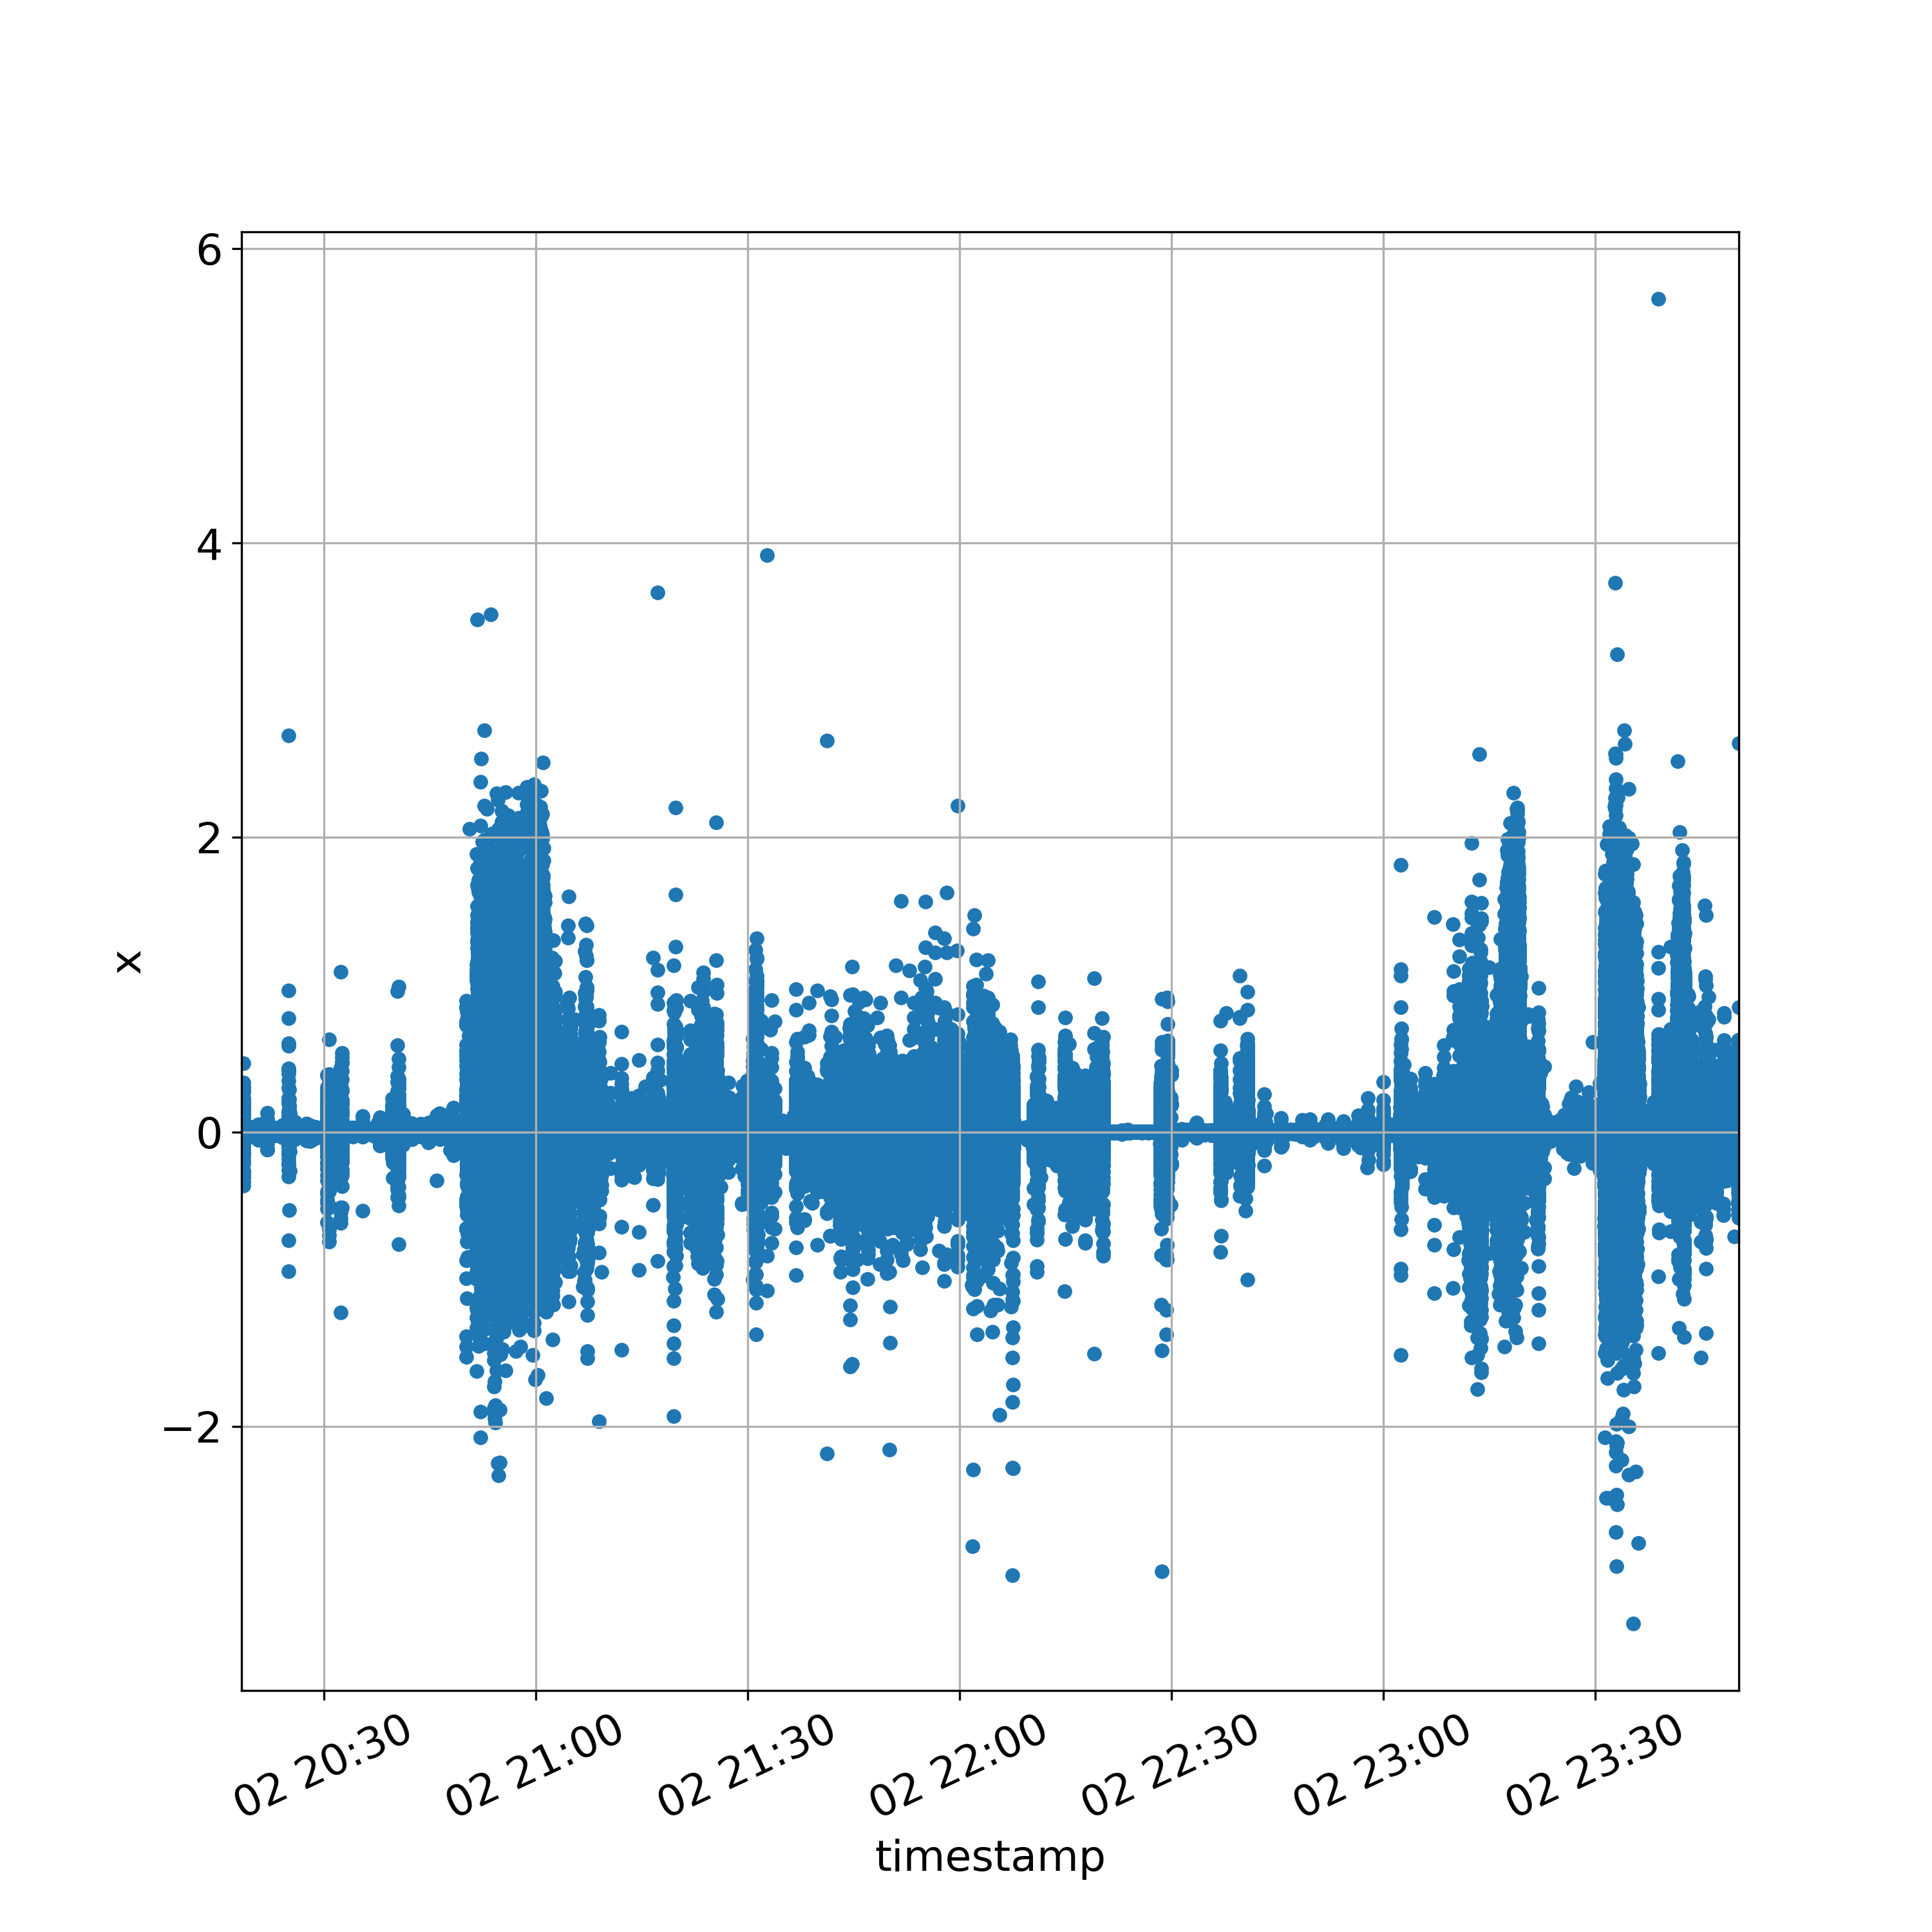
\includegraphics[width=\textwidth]{DC6359_full_x}
		\caption{Accelerometer}
		\label{fig:acc-chunk}		
	\end{subfigure}\hfill%
	\begin{subfigure}[c]{0.49\columnwidth}
		\centering
		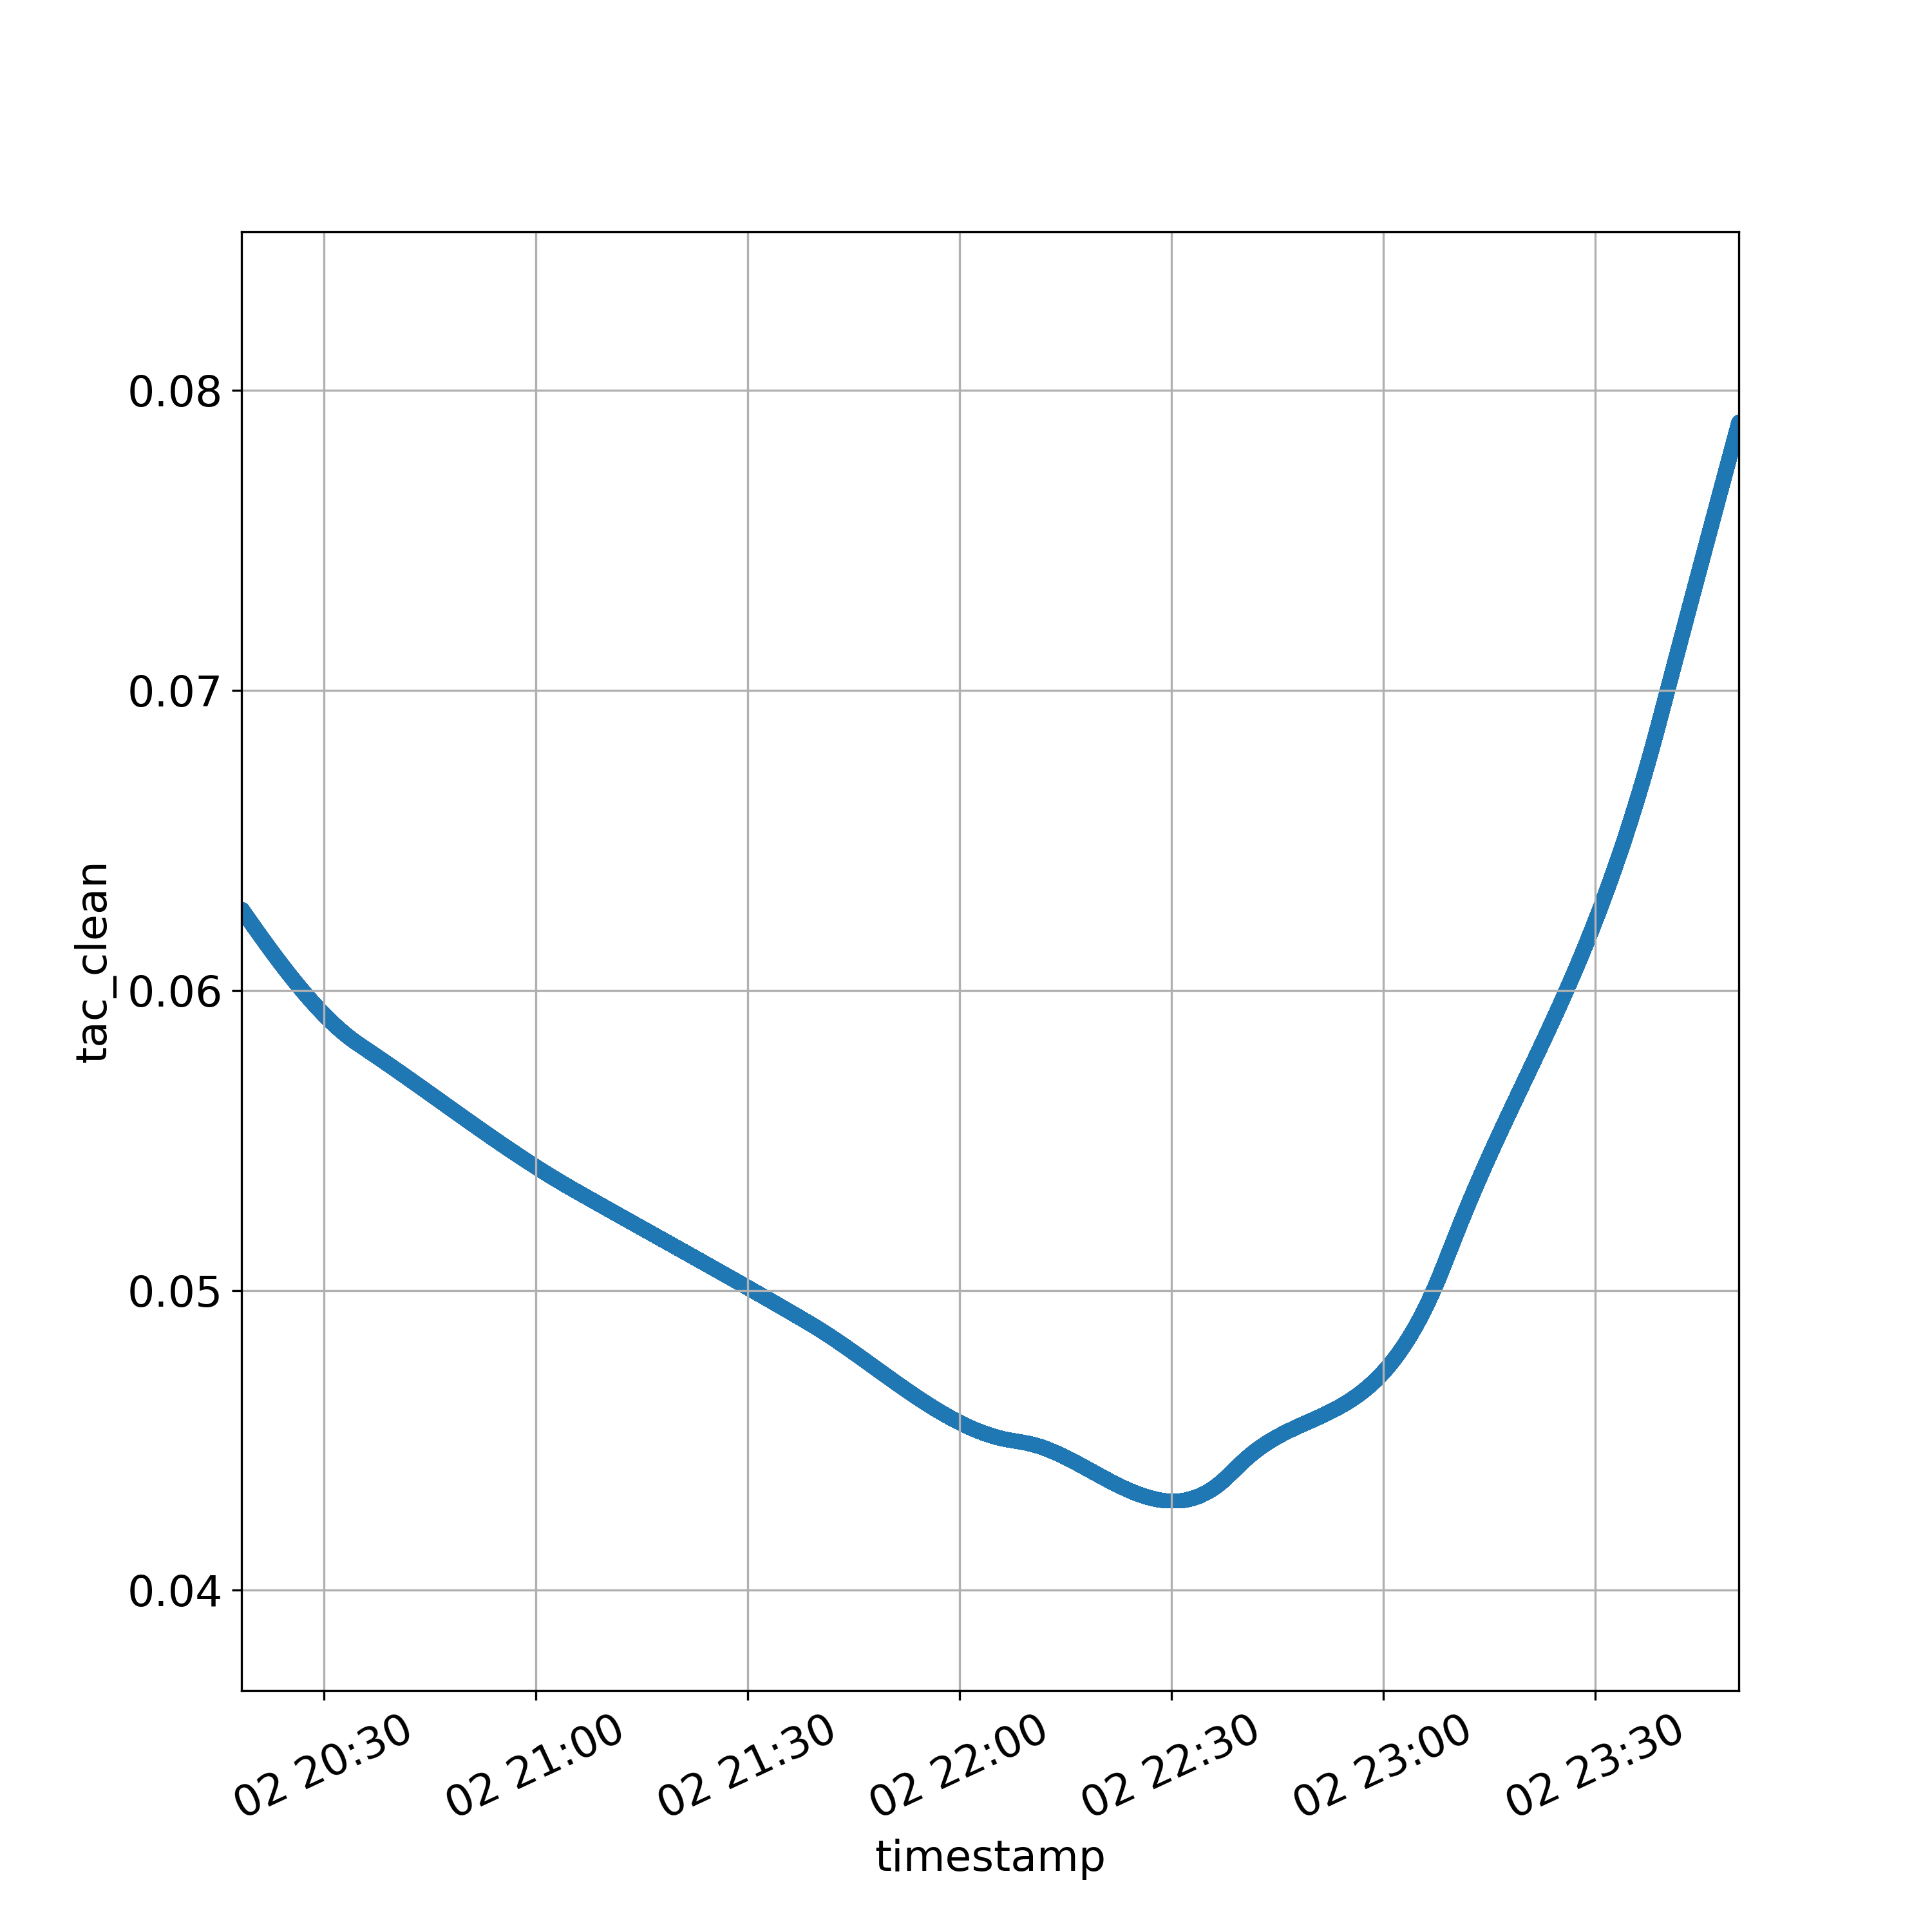
\includegraphics[width=\textwidth]{DC6359_full_clean}
		\caption{TAC}
		\label{fig:tac-chunk}
	\end{subfigure}
	\caption{Chunks of final splitted data for sample \texttt{DC6359}}
\end{figure}

%### Artificial vs Real data...
%### More Detail about the methods



\section{Method}\label{sec:method}
In order to process the accelerometer and TAC value timeseries data, an approach dealing with the continuous data stream over time is required.
Since almost all machine learning approaches require an input of constant length, a technique such as the sliding window time series analysis, combined with sequence padding, can be used.
This method enables the analysis on fractions of the time series data with a constant length.
The sliding window therefore partitions the data into a number of finite-length segments and tries to relate $ws$ past data points to a prediction $y$ by grouping \cite{MOZAFFARI2015150}.
The sliding window is defined by the parameters windows size ($ws$) and the stride size ($ss$).
So at any given point $t_n$ in time $t$, the subset tuple 

\begin{equation}
	s_{t_n} = (\{ x_{t_{n - i}}, x \in X, ws > i \geq 0 \}, y_{t_n})
\end{equation}

is calculated.
As all data points are evenly spaced out due to the resampling, we do not have to take the elapsed time between observations into account.
The stride indicates the increment of $n$ for $t_n$.
For this regression, a window size of $10\si{\second}$ and a stride of $2\si{\second}$ was used.
The window size was chosen as in \cite{DBLP:conf/ijcai/KillianPNMC19} and the stride values were determined experimentally in order to create a feasible amount of data to work with that could still represent motion and does lack specific scientific justification.
















\subsection{Feature Extraction}\label{ssec:feature}
By applying the sliding window with the parameters as stated above on the data resampled at $40 \si{\hertz}$, this results in a feature matrix of $400 \times 3$ features. In order to reduce the amount of data and increase the information at the same time, a manual feature extraction phase was implemented.
The extracted features are shown in table \ref{tab:features}. Principal component analysis (PCA) is used for dimensionality reduction to avoid issues like overfitting. The three-dimensional accelerometer data is reduced into one dimension by using the PCA class from  \texttt{scikit-learn} \cite{scikit-learn}.

\begin{table}[h]
	\resizebox{\columnwidth}{!}{%
		\centering
		\begin{tabular}{|l|c|l|}
			\hline
			Features & Generated data & Definition\\
			\hline
			
			First & 3 & The first elements per axis\\
			Last & 3 & The last elements per axis\\
			Mean & 3 & The mean per axis\\
			Median & 3 & The median per axis\\
			Var & 3 & The variation per axis\\
			Std & 3 & The standard deviation per axis\\
			Min & 3 & The minimum per axis\\
			Max & 3 & The maximum per axis\\
			Argmin & 3 & The index of the minimum per axis\\
			Argmax & 3 & The index of the maximum per axis\\
			Sum & 3 & The sum per axis\\
			Q50 & 3 & The 50\% quantile per axis\\
			Q75 & 3 & The 75\% quantile per axis\\
			Q25 & 3 & The 25\% quantile per axis\\
			PCA & 400 & The principal component value of all 3 axis\\
			MinPCA & 1 & The minimum of PCA\\
			MaxPCA & 1 & The maximum of PCA\\
			MeanPCA & 1 & The mean of PCA\\
			
			
			\hline
		\end{tabular}
	}
	\caption{Features extracted per sliding window dataframe.}
	\label{tab:features}
\end{table}

Additional parameters have been extracted using \texttt{tsfresh} \cite{DBLP:journals/ijon/ChristBNK18}, but not all algorithms have been trained with the additional features due to runtime constraints.

\begin{table}[h]
	\resizebox{\columnwidth}{!}{%
		\centering
		\begin{tabular}{|l|c|l|}
			\hline
			Features & Generated data & Description \\
			\hline
			
			abs\_energy & 3 & \href{https://tsfresh.readthedocs.io/en/latest/api/tsfresh.feature_extraction.html\#tsfresh.feature_extraction.feature_calculators.abs_energy}{absenergy per axis}\\
			absolute sum of changes & 3 & \href{https://tsfresh.readthedocs.io/en/latest/api/tsfresh.feature_extraction.html\#tsfresh.feature_extraction.feature_calculators.abs_energy}{absolute sum of changes per axis}\\
			autocorrelation & 3 & \href{https://tsfresh.readthedocs.io/en/latest/api/tsfresh.feature_extraction.html\#tsfresh.feature_extraction.feature_calculators.autocorrelation}{autocorrelation per axis}\\
			binned\_entropy & 3 & \href{https://tsfresh.readthedocs.io/en/latest/api/tsfresh.feature_extraction.html\#tsfresh.feature_extraction.feature_calculators.binned_entropy}{binned entropy per axis}\\
			c3 & 3 & \href{https://tsfresh.readthedocs.io/en/latest/api/tsfresh.feature_extraction.html\#tsfresh.feature_extraction.feature_calculators.c3}{c3 per axis}\\
			cid\_ce & 3 & \href{https://tsfresh.readthedocs.io/en/latest/api/tsfresh.feature_extraction.html\#tsfresh.feature_extraction.feature_calculators.cid_ce}{cid ce per axis}\\
			count\_above & 3 & \href{https://tsfresh.readthedocs.io/en/latest/api/tsfresh.feature_extraction.html\#tsfresh.feature_extraction.feature_calculators.count_above}{count above per axis}\\
			count\_above\_mean & 3 & \href{https://tsfresh.readthedocs.io/en/latest/api/tsfresh.feature_extraction.html\#tsfresh.feature_extraction.feature_calculators.count_above_mean}{count above mean per axis}\\
			count\_below & 3 & \href{https://tsfresh.readthedocs.io/en/latest/api/tsfresh.feature_extraction.html\#tsfresh.feature_extraction.feature_calculators.count_below}{count below per axis}\\
			count\_below\_mean & 3 & \href{https://tsfresh.readthedocs.io/en/latest/api/tsfresh.feature_extraction.html\#tsfresh.feature_extraction.feature_calculators.count_below_mean}{count below mean per axis}\\
			first\_location\_of\_maximum & 3 & \href{https://tsfresh.readthedocs.io/en/latest/api/tsfresh.feature_extraction.html\#tsfresh.feature_extraction.feature_calculators.first_location_of_maximum}{first location of maximum per axis}\\
			first\_location\_of\_minimum & 3 & \href{https://tsfresh.readthedocs.io/en/latest/api/tsfresh.feature_extraction.html\#tsfresh.feature_extraction.feature_calculators.first_location_of_minimum}{first location of minimum per axis}\\
			kurtosis & 3 & \href{https://tsfresh.readthedocs.io/en/latest/api/tsfresh.feature_extraction.html\#tsfresh.feature_extraction.feature_calculators.kurtosis}{kurtosis per axis}\\
			last\_location\_of\_maximum & 3 & \href{https://tsfresh.readthedocs.io/en/latest/api/tsfresh.feature_extraction.html\#tsfresh.feature_extraction.feature_calculators.last_location_of_maximum}{last location of maximum per axis}\\
			last\_location\_of\_minimum & 3 & \href{https://tsfresh.readthedocs.io/en/latest/api/tsfresh.feature_extraction.html\#tsfresh.feature_extraction.feature_calculators.last_location_of_minimum}{last location of minimum per axis}\\
			longest\_strike\_above\_mean & 3 & \href{https://tsfresh.readthedocs.io/en/latest/api/tsfresh.feature_extraction.html\#tsfresh.feature_extraction.feature_calculators.longest_strike_above_mean}{longest strike above mean per axis}\\
			longest\_strike\_below\_mean & 3 & \href{https://tsfresh.readthedocs.io/en/latest/api/tsfresh.feature_extraction.html\#tsfresh.feature_extraction.feature_calculators.longest_strike_below_mean}{longest strike below mean per axis}\\
			mean\_abs\_change & 3 & \href{https://tsfresh.readthedocs.io/en/latest/api/tsfresh.feature_extraction.html\#tsfresh.feature_extraction.feature_calculators.mean_abs_change}{mean abs change per axis}\\
			mean\_change & 3 & \href{https://tsfresh.readthedocs.io/en/latest/api/tsfresh.feature_extraction.html\#tsfresh.feature_extraction.feature_calculators.mean_change}{mean change per axis}\\
			mean\_second\_derivative\_central & 3 & \href{https://tsfresh.readthedocs.io/en/latest/api/tsfresh.feature_extraction.html\#tsfresh.feature_extraction.feature_calculators.mean_second_derivative_central}{mean second derivative central per axis}\\
			number\_crossing m & 3 & \href{https://tsfresh.readthedocs.io/en/latest/api/tsfresh.feature_extraction.html\#tsfresh.feature_extraction.feature_calculators.number_crossing_m}{number crossing m per axis}\\
			number\_peaks & 3 & \href{https://tsfresh.readthedocs.io/en/latest/api/tsfresh.feature_extraction.html\#tsfresh.feature_extraction.feature_calculators.number_peaks}{number peaks per axis}\\
			skewness & 3 & \href{https://tsfresh.readthedocs.io/en/latest/api/tsfresh.feature_extraction.html\#tsfresh.feature_extraction.feature_calculators.skewness}{skewness per axis}\\
			time\_reversal\_asymmetry\_statistic & 3 & \href{https://tsfresh.readthedocs.io/en/latest/api/tsfresh.feature_extraction.html\#tsfresh.feature_extraction.feature_calculators.time_reversal_asymmetry_statistic}{time reversal asymmetry statistic per axis}\\
			variation\_coefficient & 3 & \href{https://tsfresh.readthedocs.io/en/latest/api/tsfresh.feature_extraction.html\#tsfresh.feature_extraction.feature_calculators.variation_coefficient}{variation coefficient per axis}\\
			\hline
		\end{tabular}
	}

	\caption{Additional features extracted using \texttt{tsfresh} \cite{DBLP:journals/ijon/ChristBNK18}.}
	\label{tab:features-additional}
\end{table}



In comparison to \cite{DBLP:conf/ijcai/KillianPNMC19}, a few things are handled differently already: first, all of the above features are calculated on the whole window, while \citeauthor{DBLP:conf/ijcai/KillianPNMC19} used a two-tiered window approach, a short-term and a long-term window, and some additional features, that were calculated separately \cite{DBLP:conf/ijcai/KillianPNMC19}.
Secondly, \citeauthor{DBLP:conf/ijcai/KillianPNMC19} extracted features more specific to audio analysis.
Their features sum up to $1215$ data points, while we currently extract $445$ with $72$ additional \texttt{tsfresh} features, creating a total of $517$. 
This already shows a significant difference between the methods used and introduces additional obstacles for comparison.














\subsection{Hyperparameter Optimization}\label{ssec:hpo}
In order to create the best possible regressor, another important element besides feature extraction is the tuning of said model. 
While parameters are learned during training – for example the slope of linear regression or weights of neural network, hyperparameters can be arbitrarily set by a data scientist beforehand.



\begin{figure}[h]
	\centering
	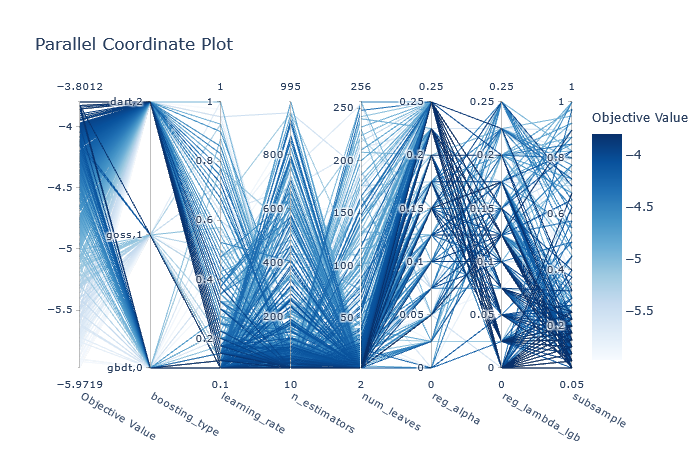
\includegraphics[width=\columnwidth]{hpo-parallel}
	\caption{Exemplary HPO value plot for \texttt{LightGBM} with sample \texttt{JB3156} chunk 0}
	\label{fig:hpo-parallel}
\end{figure}



Therefore, the selection of correct values for these hyperparameters is crucial and can significantly improve the performance of a model.
This tuning process can be viewed as a type of optimization problem itself cause we aim to find the right combination of a set of hyperparameters to e.g. minimize the loss or maximize the performance metric.
Apart from a manual search, random search and grid search are viable options.
However, such an approach is more or less equal to a brute force attempt.
Hence, so called automated hyperparameter optimization (HPO) algorithms have evolved, using techniques such as bayesian optimization, gradient descent and evolutionary algorithms.
This enables efficiently searching large spaces and pruning of unpromising trials for faster results.


Multiple libraries can be used; most famous contenders \texttt{Hyperopt} \cite{DBLP:conf/icml/BergstraYC13} and \texttt{Optuna} \cite{DBLP:conf/kdd/AkibaSYOK19} are subject of countless articles comparing them (e.g. \cite{neptune_2019}). \texttt{Optuna} was chosen based on the better documentation and build-in visualization.


A hyperparameter optimization study was performed separately for each of the algorithms presented in \ref{ssec:algorithms}.
Figure \ref{fig:hpo-parallel} shows a value plot for different hyperparameters for the \texttt{LightGBM} \cite{DBLP:conf/nips/KeMFWCMYL17} algorithm, validated the chunk number $0$ of sample \texttt{JB3156}.
This dataset was chosen because it is the largest file after splitting.

Depending on the runtime of the algorithm and the respective features, each study was optimized for $100 - 1000$ trials.


\begin{figure*}[bt]
	\centering
	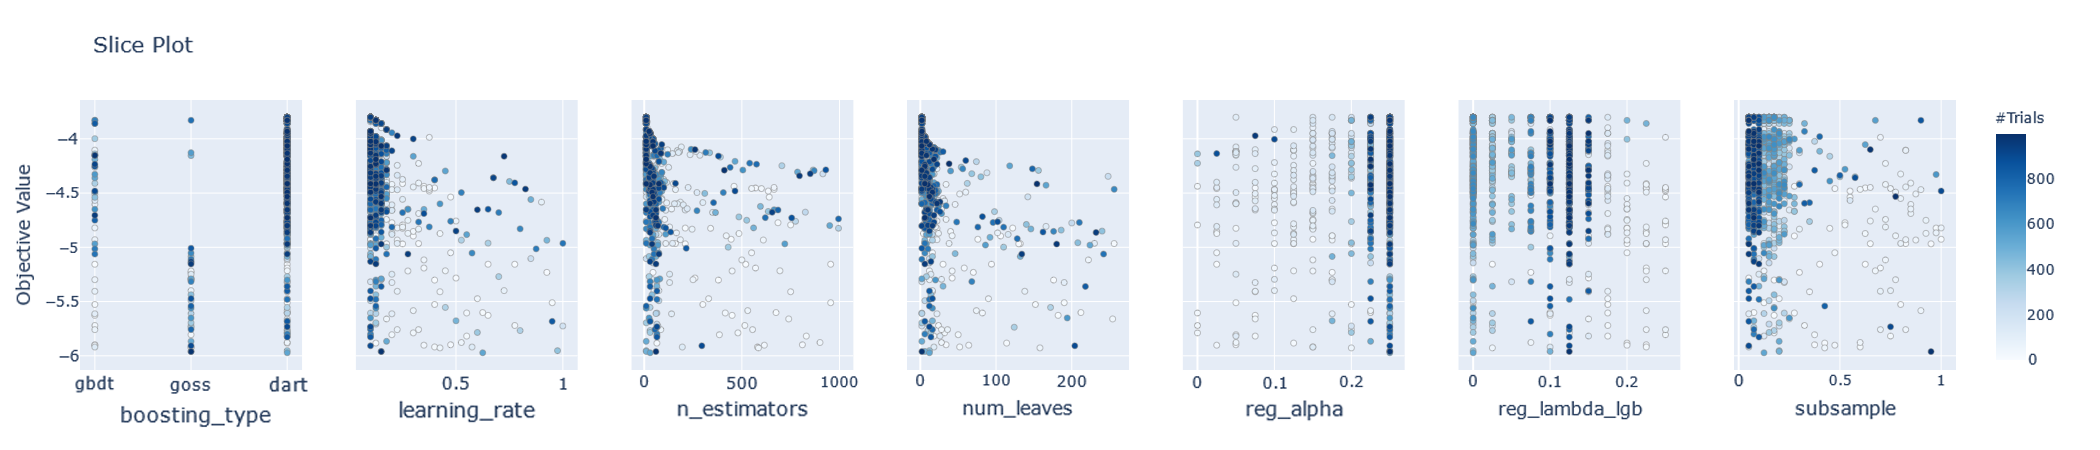
\includegraphics[width=\textwidth]{hpo-sliceBIG}
	\caption{Exemplary HPO slice plot for \texttt{LightGBM} with sample \texttt{JB3156} chunk 0}
	\label{fig:hpo-slice}
\end{figure*}

\begin{figure}[h]
	\centering
	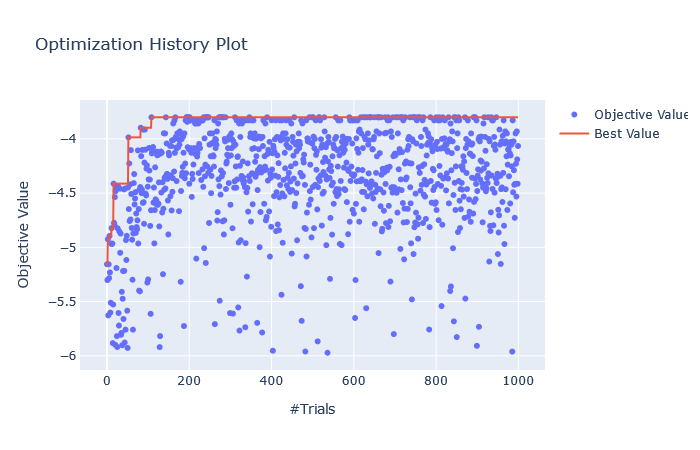
\includegraphics[width=\columnwidth]{hpo-hist}
	\caption{Exemplary HPO history plot for \texttt{LightGBM} with sample \texttt{JB3156} chunk 0}
	\label{fig:hpo-hist}
\end{figure}

Figure \ref{fig:hpo-slice} shows the variation of each hyperparameter over time.
Whereas the final optimization history is shown in figure \ref{fig:hpo-hist}.
This graph already clearly indicates, that the optimization reached a plateau quite fast and was unable to significantly improve the performance further on.
In case that this model can not satisfy the desired performance requirements, further work in \ref{ssec:feature} is needed.










\subsection{Algorithms}\label{ssec:algorithms}
In ensemble learning theory, we call weak learners (or base models) models that can be used as building blocks for designing more complex models by combining several of them.
Most of the time, these basics models perform not so well by themselves either because they have a high bias often due to low degree of freedom models or because they have too much variance to be robust in case of high degree of freedom models.
But a low bias and a low variance, although they most often vary in opposite directions, are the two most fundamental features expected for a model. 
This is the well known bias-variance tradeoff.

So the idea of ensemble methods is to try reducing bias and/or variance of such weak learners by combining several of them together in order to create a strong learner (or ensemble model) that achieves better performances than any algorithm alone.
One can combine these models in different ways; three major kinds are known in literature: bagging to decrease the model’s variance, boosting decreasing the model’s bias, and stacking to increasing the predictive force of the classifier.

Thus, in consideration of our research question, the algorithms used all implement the concept of ensemble learning.
We evaluated \texttt{ExtraTrees}, \texttt{RandomForest}, \texttt{AdaBoost}, \texttt{GradientBoosting}, and \texttt{HistGradientBoosting} from the popular \texttt{scikit-learn} library \cite{scikit-learn} to establish a baseline for better comparison.

Nonetheless, one of the most popular shallow learning techniques in recent years has been gradient boosting, dominating many Kaggle (subsidiary of Google LLC, online community of data scientists and machine learning practitioners) competitions with heterogeneous tabular data.
Similar to random forest, gradient boosting works by ensembling many decision trees in order to perform regression or classification.
However, unlike random forest, gradient boosting grows trees sequentially, iteratively growing trees based on the residuals of the previous tree.
Doing so allows gradient boosting to focus on particularly tricky observations and yields an extraordinarily powerful ensemble of trees.
Among the most common algorithms in recent years are \texttt{XGBoost} \cite{DBLP:conf/kdd/ChenG16}, \texttt{LightGBM} \cite{DBLP:conf/nips/KeMFWCMYL17} and \texttt{CatBoost} \cite{DBLP:journals/corr/abs-1810-11363}.

All used algorithms share an implementation of the \texttt{scikit-learn} API \cite{sklearn_api}, which made it easy to use a shared infrastructure.


\section{Results}
In table \ref{tab:mse} the mean squared error (MSE) of all trained models is shown. Clearly these errors are quite low, but in the context of our regression model the error is naturally quite low, because the mean squared error is not a relative value but an absolute value and depends on the value range which, in our case, is small. 

\begin{table}[h]
	\resizebox{.65\columnwidth}{!}{%
		\centering
		\begin{tabular}{|l|c|}
			\hline
			Model & MSE \\
			\hline
			ETS & 0.005806121997238007 \\
			HGB & 0.006537057262386852 \\
			LGB & 0.006659725937704261 \\
			XGB & 0.009520274940766137 \\
			\hline
		\end{tabular}
	}
	\caption{Mean squared error of trained models}
	\label{tab:mse}
\end{table}

In the figure \ref{fig:predictions} the orange lines represent our prediction and the blue lines represent the ground truth. With these figures it is quite clear why the mean squared error value needs to be even lower.

\begin{figure*}[bt]
	\begin{subfigure}{.24\textwidth}
		\centering
		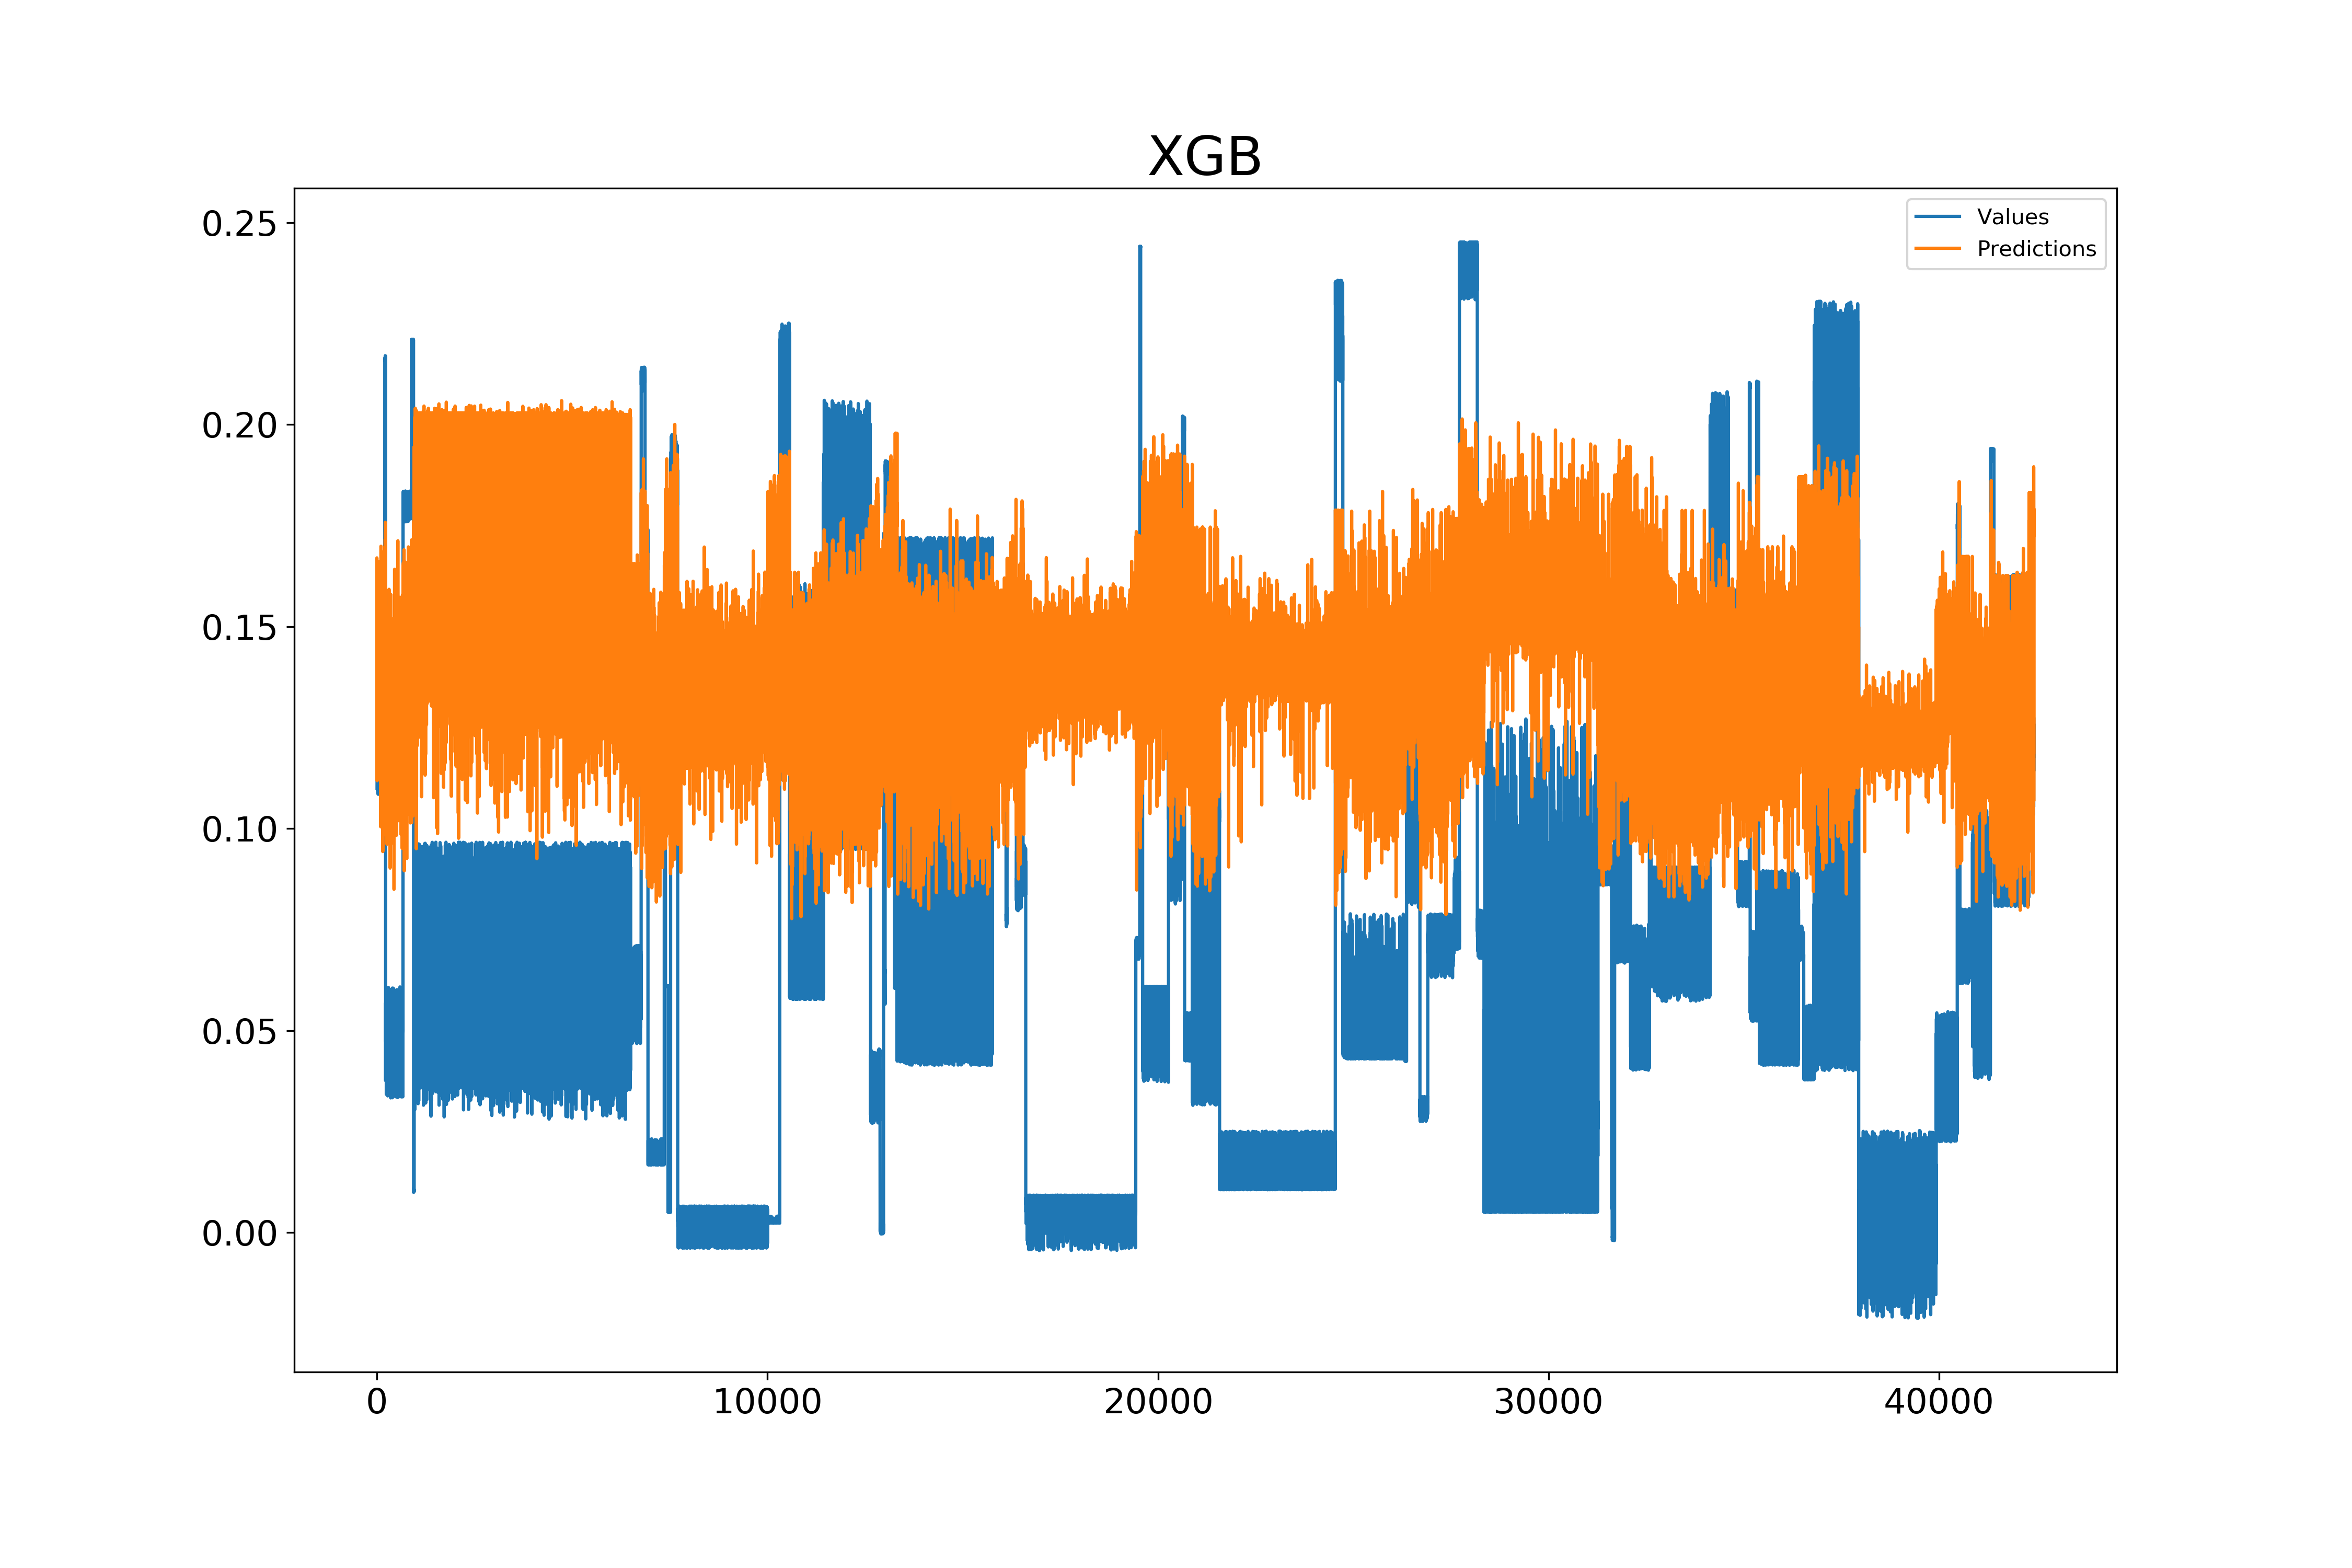
\includegraphics[width=\textwidth]{XGB_results}
		\caption{XGBoost}
	\end{subfigure}
	\begin{subfigure}{.24\textwidth}
		\centering
		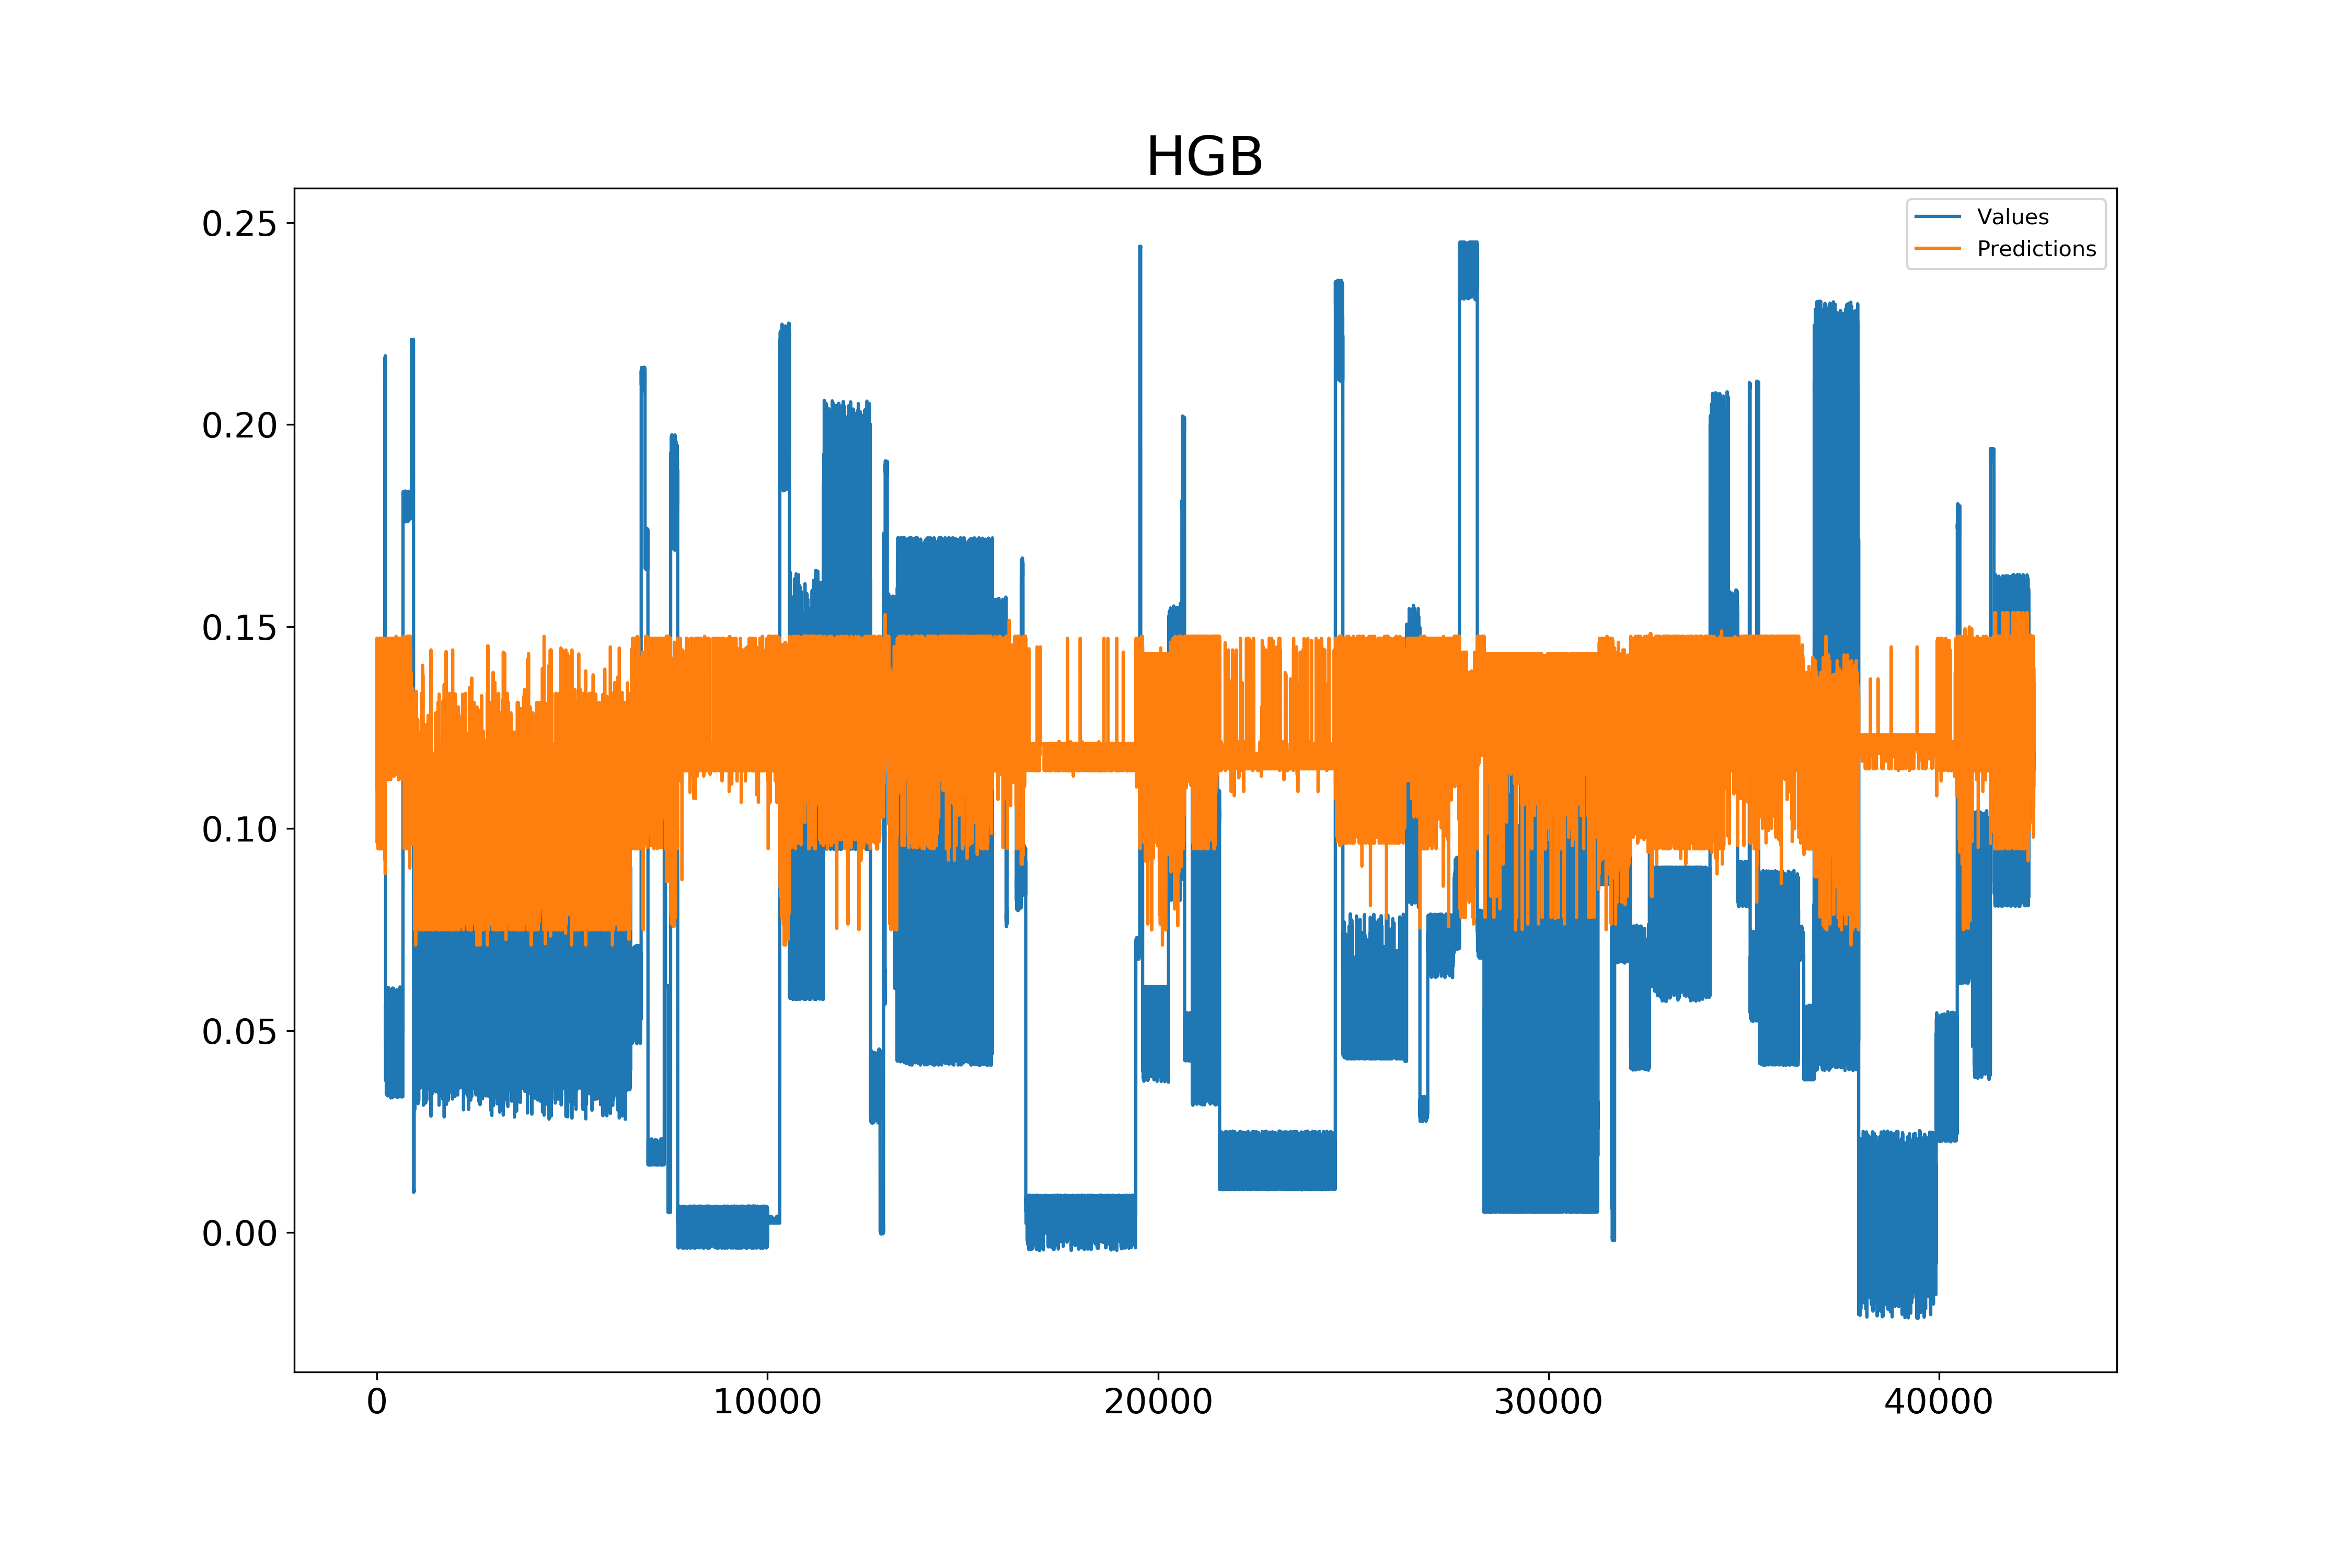
\includegraphics[width=\textwidth]{HGB_results}
		\caption{HistoryGradientBoosting}
	\end{subfigure}
	\begin{subfigure}{.24\textwidth}
		\centering
		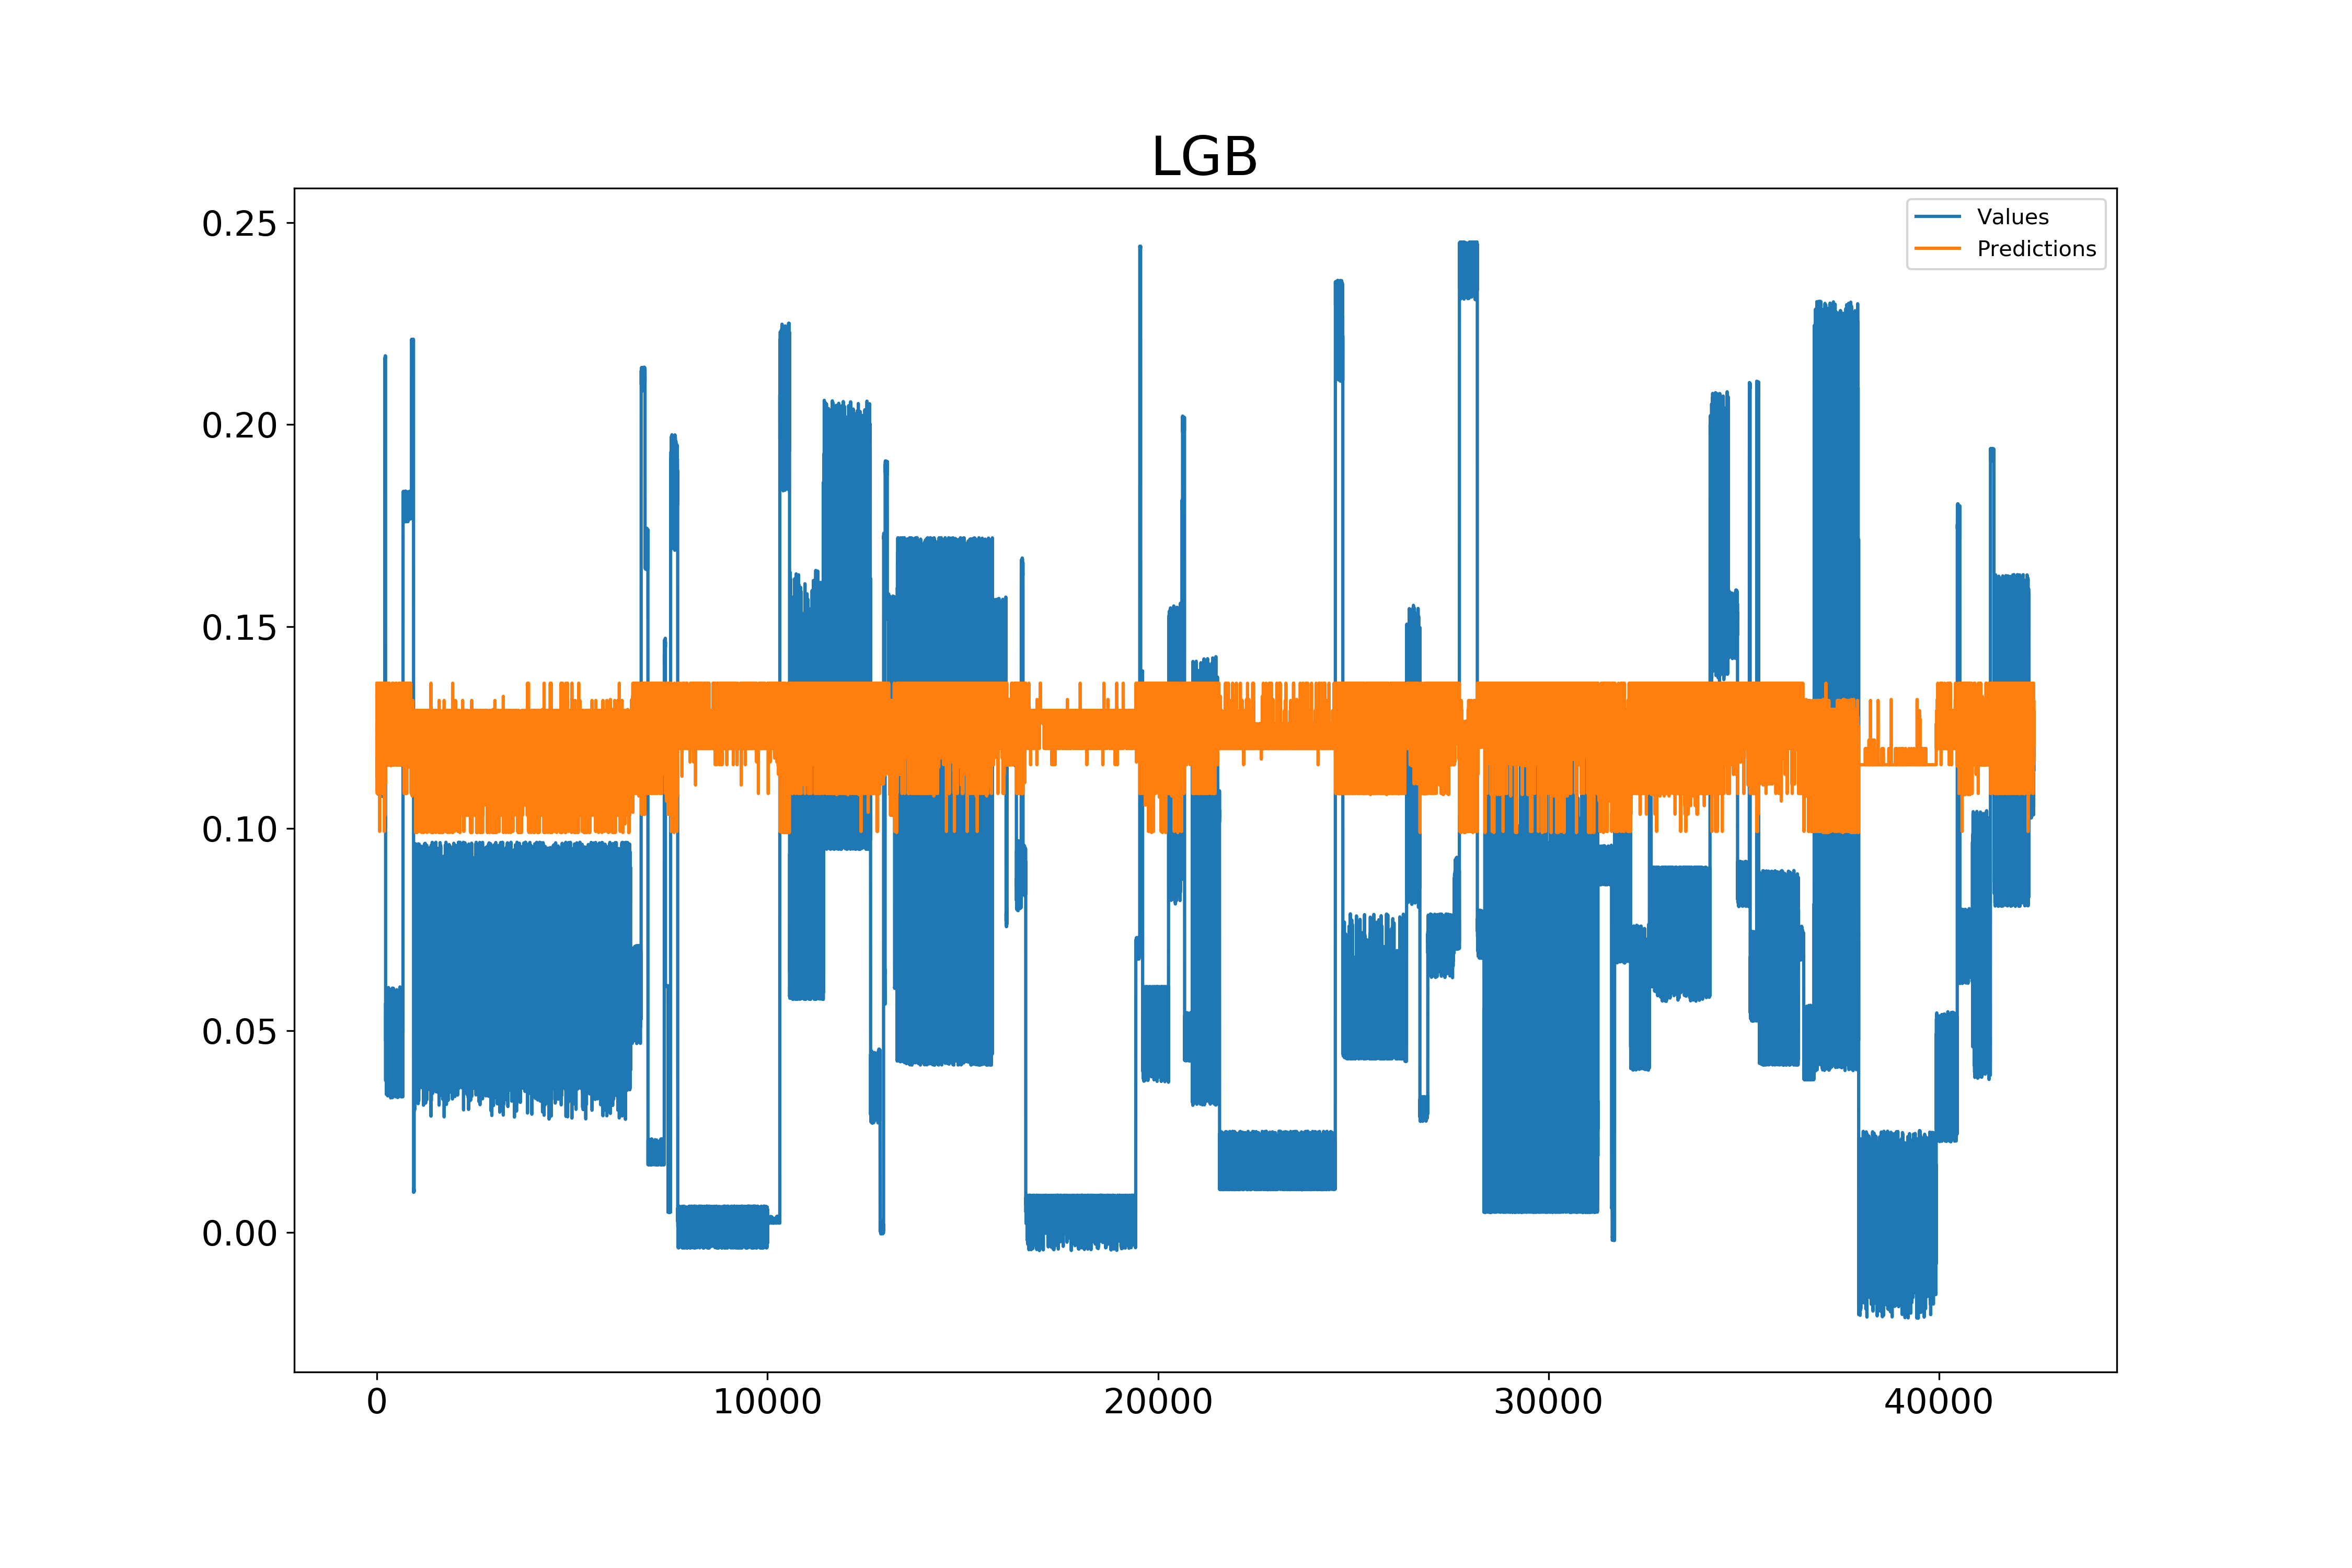
\includegraphics[width=\textwidth]{LGB_results}
		\caption{LightGBM}
	\end{subfigure}
	\begin{subfigure}{.24\textwidth}
		\centering
		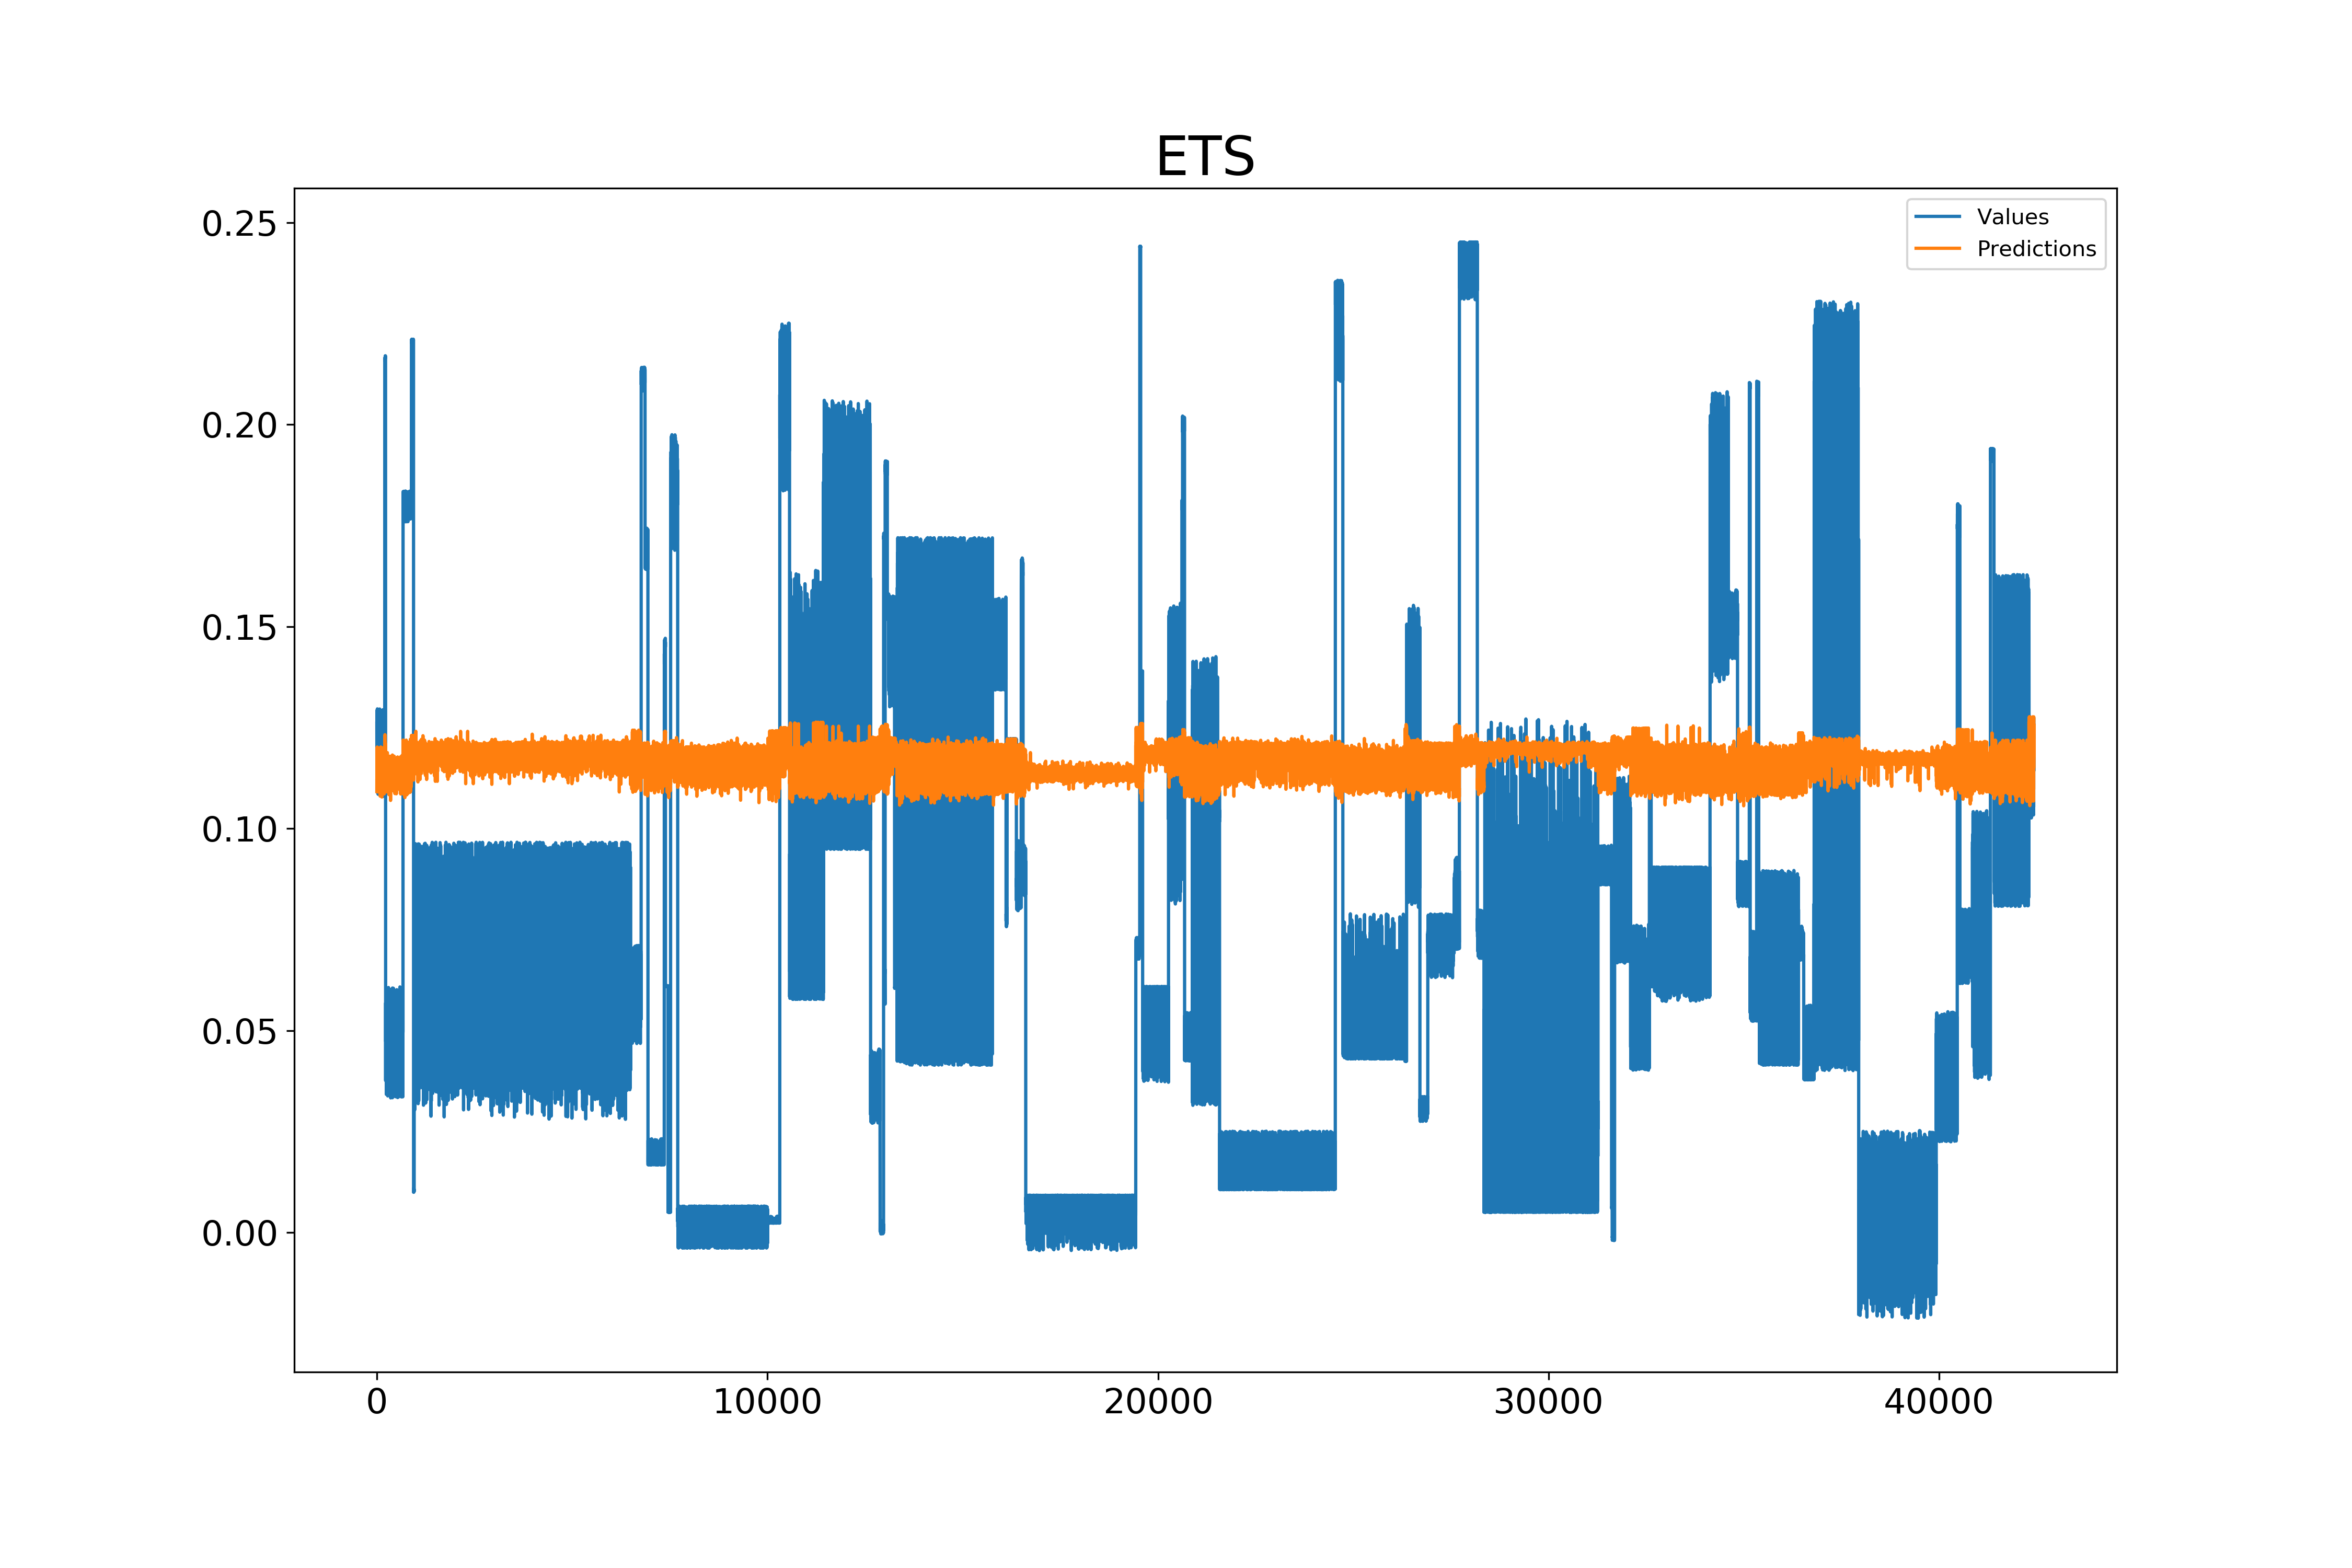
\includegraphics[width=\textwidth]{ETS_results}
		\caption{ExtraTrees}
	\end{subfigure}
	\caption{Comparison of concatenated predictions (orange) to ground truth (blue).}
	\label{fig:predictions}
\end{figure*}

Our results show that the regression is not able to differentiate between below and above the legal limit with the features extracted.

\subsection{Discussion}
We had a deadline to submit our results and in the mean time, the project continued to scale up as we progressed through different stages.
Thus, we had to compromise a bit of quality to gain speed and finish our project on time. These difficulties and compromises include the feature extraction where we could use more promising signal processing approaches to obtain better results.
More detailed description of this matter is further explained in the section \ref{sec:futurework}.

In the case of an application like this to become publicly accessible to users, there comes great responsibility with the data collection of the owners.
For one, this is extremely sensible data that could be trained to recognize even further information about an individual.
Another point is that in case the TAC level data gets leaked or sold to a third party, it could be abused to target the user with relevant ads or give drunk users higher transportation fares.
And finally, the app itself could produce defective detections, like a false negative resulting in irresponsible behavior while depending on a feedback from the application as an excuse to drive, for example.       

A direct comparison of the results of our trained regression model to the model proposed in \cite{DBLP:conf/ijcai/KillianPNMC19} is not possible, because not only did they not specify, on which chunks of the dataset they tested their trained models, they also performed a classification. And our regression has a more precise output and that results in worse metrics for our model, but does not necessarily represent the performance, because a threshold could be undershot by a tiny amount and would not necessarily mean a worse result, just a more precise one.

In addition to the aforementioned points, because this paper was created during a university course, many of our expectations couldn't be met because of strict time constraints.
If more time was available we could have increased our model performance by using details we discussed in the beginning of this section and chapter \ref{sec:futurework}.

\subsection{Conclusion}
Overall this project was a huge learning experience for all of us, and we learned a lot about data analysis. Additionally, we learned how fast a project can grow in dimension by adding more complexity and data. Furthermore we can conclude that in shallow machine learning algorithms the feature extraction has a huge impact on the model performance.

Our results were not meeting our expectations, but were of course limited by the time constraints of a university project and lacking the computational power to train more  models with the proposed changes. Otherwise, we see our whole pipeline of data analysis, cleaning and model tuning as a huge success.

\section{Future Work}\label{sec:futurework}
For future work we formulate some specific ideas to further improve our machine learning model and the usability for end users.
On one hand we've created an android application prototype, which can read the accelerometer data readings which are needed when using our model.

Improving the machine learning model presented in this paper could be done in several ways. One way could be to extract even more features, specifically using the accelerometer data as signal data and extract more audio features such as: Continuous wavelet transform, Mel-frequency cepstrum and many more. Together with extracting different statistical features the result could be improved and features that are deemed more usable for our regression can be used. Similarly, analyzing the accelerometer data could also be used to extract features that for example indicate if the participant is walking, sitting or standing. And finally, features with a low correlation could be removed.

Additionally, a new dataset could be collected by recreating the original application from \cite{DBLP:conf/ijcai/KillianPNMC19} and eliminating some shortfalls they had in collecting the data, e.g. loss of phone power, missing or completely unusable data points. Furthermore, using a more solid method of collecting either the transdermal or blood alcohol content could be used and more features could be collected, such as if the participant is taking a drink or if he is present in a bar.

Varying the sliding window length and step size could improve the regression. Using a bigger value range for the hyperparameter optimization and more trials could also help to improve the results as well. And last but not least, evaluating other types of machine learning algorithms such as deep learning models with LSTM cells is feasible. 

%% The next two lines define the bibliography style to be used, and
%% the bibliography file.
\bibliographystyle{ACM-Reference-Format}
\bibliography{bibliography}

\end{document}
\endinput
%%
%% End of file `sample-sigconf.tex'.
